\chapter{Preliminaries}
\label{ch:preliminaries}

\section{Tabular Data}
\label{ch:preliminaries-dataSynthesis-tabularData}

Tabular data is one of the most common forms of structured data \cite{hernandez2022SyntheticDataGeneration} used to store, classify and share information \cite{pilaluisa2022ContextualWordEmbeddings}.
A table is made up of individual cell entries stored in rows and columns.
Rows can be seen as unique data points, and columns as their different features \cite{borisov2022DeepNeuralNetworks, yoon2020VIMEExtendingSuccess}.
This format is the most common way to maintain massive databases \cite{esmaeilpour2022BidiscriminatorGANTabular, yoon2020VIMEExtendingSuccess}, and is crucial for applications that store heterogeneous information such as demographics, medical or financial information \cite{borisov2022DeepNeuralNetworks, yoon2020VIMEExtendingSuccess}.
Tabular data consists of multiple attribute types, such as categorical or continuous data types \cite{borisov2022DeepNeuralNetworks}.
From a statistical perspective, quantitative and qualitative variables are to be differentiated \cite{lane2003IntroductionStatistics}.
Quantitative variables are variables that can be measured numerically and express a specific quantity or amount. 
Qualitative variables cannot be measured numerically but describe qualities or characteristics that do not have any ordering  \cite{lane2003IntroductionStatistics}. 
These variables are divided into categories or groups based on shared attributes. 
The categories are usually non-numerical and consist of words or labels, such as gender (\textit{male}, \textit{female}) or hair color (\textit{blonde}, \textit{brunette}, \textit{red}, etc.) and may be assigned to numbers.

Quantitative variables can be further subdivided into continuous or discrete variables.
Continuous variables can take on an infinite number of values within a specific range. 
These variables are often measured on a continuous scale, can have decimal or fractional parts, and are stored as a numerical data type \cite{lane2003IntroductionStatistics, lederrey2022DATGANIntegratingExperta}.
Discrete variables are also numbers, but they can only have a specific and limited number of unique values within a certain range. 
They are usually expressed as whole natural numbers (or integers) and are commonly used for counting or listing items. \cite{lane2003IntroductionStatistics}.

Qualitative variables are often called categorical values and can be further classified into binary or nominal types \cite{lane2003IntroductionStatistics}.
Binary variables have only two possible outcomes (\eg booleans with \textit{True} or \textit{False}), while nominal variables consist of at least three distinct values that do not follow a specific order \cite{lederrey2022DATGANIntegratingExperta, lane2003IntroductionStatistics}.

\newpage
This work adapts the formal definition of a table from \cite{xu2019ModelingTabularData}:

\begin{displayquote}
A table \textbf{$T$} contains $N_q$ qualitative (categorical) columns $\{Q_1, \dots, Q_{N_q}\}$ and $N_p$ quantitative columns $\{P_1, \dots, P_{N_p}\}$, 
where the quantitative columns consist of both continuous and discrete variables. 
Each column is considered to be a random variable. 
These random variables follow an unknown joint distribution $\mathbb{P}(Q_{1:N_q}, P_{1:N_p})$. 
One row $r_j = \{q_{1,j}, \dots, q_{N_q,j}, p_{1,j}, \dots, p_{N_p,j}\}$, $j \in \{1, \dots, n\}$, is one observation from the joint distribution.
\end{displayquote}

The term "table" as described in this definition aligns with the concept of a single "table" or "relation" as described in the classical relational model \cite{codd1970RelationalModelData} commonly used in modern relational databases \cite{w.eembley2009RelationalModel}.
Essentially, this definition takes a probabilistic view of the table in a relational database.
Rather than viewing the data within the table as static or independent values, it perceives them as elements derived from an unseen, underlying probability distribution.
This is an important perspective for statistical analysis and machine learning tasks on database content.

\cite{codd1970RelationalModelData}

For consistency and simplicity, this thesis will further refer to qualitative columns as \textit{categorical} and to quantitative columns as \textit{continuous} or \textit{numerical}. 
Discrete values are not separately mentioned but should be considered included in \textit{continuous}/\textit{numerical} columns.

It is also possible that tabular data contains other particular data types like dates or timestamps, which often include information on the specific time a datapoint was recorded \cite{hernandez2022SyntheticDataGeneration}.
This kind of tabular data can be considered dynamic tabular data, where individual records, \ie rows, can be dependent on each other, also known as a multivariate time series \cite{padhi2021TabularTransformersModeling}.
In static tabular data, on the other hand, the individual rows are independent \cite{padhi2021TabularTransformersModeling}.
Hence, the order of rows and columns does not carry any meaning \cite{somepalli2021SAINTImprovedNeural}.
However, the individual values in one cell may vary well depending on the values of another cell \cite{lederrey2022DATGANIntegratingExperta}.
An example of such an interdependency could occur in a demographics table, where an individual's legal status may depend on their age, 
for example, a person under 18 years of age could be considered a minor and has different legal rights and responsibilities than an adult.

The authors of \cite{borisov2022DeepNeuralNetworks} identify four possible challenges when working with tabular data in a learning context.
The first challenge identified is the "low-quality" of the data \cite[p. 4]{borisov2022DeepNeuralNetworks}. 
\textcite{borisov2022DeepNeuralNetworks} identified common data quality issues from the literature, which include missing values, data noise, extreme data points, inconsistencies, class imbalances, or high dimensionality of the data after preprocessing.

Secondly the "missing or complex irregular spatial dependencies" of tabular data \cite[p. 4]{borisov2022DeepNeuralNetworks}. 
Other common data formats like images or audio are homogeneous, meaning that they consist of only one feature type \cite{borisov2022DeepNeuralNetworks}.
Since tabular data consists of multiple features made up of a mixture of categorical and numerical values, it is a heterogeneous data format with data points as rows and features as columns \cite{borisov2022DeepNeuralNetworks}.
This format presents particular challenges for neural networks when working with tabular data, as the correlations between features are often weaker due to the absence of spatial or semantic relationships commonly found in image or text data \cite{borisov2022DeepNeuralNetworks, yoon2020VIMEExtendingSuccess}.

The third challenge is the "dependency on preprocessing" \cite[p. 4]{borisov2022DeepNeuralNetworks}. 
\cite{borisov2022DeepNeuralNetworks} highlights the importance of a preprocessing and an explicit feature construction step that is necessary when working with tabular data in a deep learning context.
This preprocessing step is crucial since it not only strongly influences the performance of deep learning models \cite{gorishniy2022EmbeddingsNumericalFeatures}, it also introduces new challenges. 
Depending on the preprocessing strategy (\autoref{sec:preprocessing}), it is possible to create a very sparse feature matrix, construct a synthetic ordinal ordering of a nominal variable, or lose some information during the conversion of the data \cite{borisov2022DeepNeuralNetworks}.

The last and fourth challenge concerns the "importance of single features" \cite[p. 4]{borisov2022DeepNeuralNetworks}. 
In homogeneous data, multiple features need to change in order for the class of the data to be changed. 
For heterogeneous tabular data, a small change in one feature variable can already alter the class of the row. 
\cite{borisov2022DeepNeuralNetworks} illustrates this with the example of an image, where multiple pixels (\ie features) need to change in a coordinated manner in order to change the content (\ie class) of the image from a dog to a cat.
For tabular data, a single change in a cell can change the prediction of a predictive model \cite{borisov2022DeepNeuralNetworks}. 
Consider a model that has to predict whether an individual's income is higher or lower than US\$ 50.000 per year \cite{Dua:2019} based on the demographic information of that individual.
Switching an individual's "education" value from "Preschool" to "Doctorate" would likely cause the prediction to change from "<=50K" to ">50K".


\subsection{Tabular Data Preprocessing}
\label{sec:preprocessing}

Different data types can and should be processed into a meaningful format to be useful for deep learning models in different ways \cite{fan2020RelationalDataSynthesisa, lederrey2022DATGANIntegratingExperta}.
That is usually the first step before working with the data on any task \cite{izonin2022TwoStepDataNormalization}.
\cite{garcia2016BigDataPreprocessing} states, that data preprocessing itself consists of multiple different tasks: data cleaning, data normalization, data transformation, data integration, missing value imputation and noise identification.
While each of the preprocessing tasks in itself is important, 
\cite{fitkov-norris2012EvaluatingImpactCategorical} and \cite{gorishniy2022EmbeddingsNumericalFeatures} showed that a proper transformation of categorical and numerical entries respectively can have a significant influence on a deep learning model's performance.
\cite{xu2019ModelingTabularData} showed the importance of normalization for synthetic tabular data generation.
Since the focus of this work is on tabular data and its synthesis, the following section will highlight the most important tabular data transformation and normalization approaches.

\subsubsection{Data Transformation}
\label{sec:dataTransformation}

\textcite[p. 5]{borisov2022DeepNeuralNetworks} introduced a taxonomy for data transformation methods and subdivides the existing approaches into "Single-Dimensional Encodings" and "Multi-Dimensional Encodings".
The goal is to transform the different values a column can take and transform them into a different (numeric) representation so that it can be processed by a deep learning model.

\textbf{Single-Dimensional Encodings:}
Single-Dimensional encoding techniques encode each cell independently \cite{borisov2022DeepNeuralNetworks}.
The following approaches are common techniques to encode a categorical column entry, usually in a text format, into a numerical format.
In ordinal- (or label-) encoding, a simple mapping from each category to a numeric value occurs. 
While this introduces a synthetic ordering of potentially unordered categories, \gls{oh} encoding overcomes this issue by introducing a new vector with the length of all possible values a categorical column can take.
All values in this vector are assigned to zero except one entry which represents the category that should be encoded, which is set to one.
However, this approach can lead to high-dimensionality feature vectors if the cardinality of the unique categories in categorical columns is large.
Binary encoding tries to reduce the dimensionality by setting the vector length to a maximum of $log(c)$ for $c$ unique categorical values in a column \cite{borisov2022DeepNeuralNetworks}.
Each possible value is mapped to a number like in ordinal-encoding, starting at 0, but the number is represented as a binary vector.
As an example, the categorical values \{\textit{Germany}, \textit{USA}, \textit{France}\} would be represented as binary values \{(0,1), (1,0), (1,1)\}. 
While representing \textit{France} in a one-hot-encoding creates the vector (0,0,1) of length three, binary encoding encodes the same information into the vector (1,1) of length two, reducing the overall dimensionality of produces encodings.
The leave-one-out encoding technique is an approach to encode a categorical column based on the target column in a machine learning scenario \cite{borisov2022DeepNeuralNetworks}. 
A categorical entry is replaced by the mean of the target variable of all rows where the same category is present, excluding the target value of the to be encoded value.
Lastly, a hash-based approach is worth mentioning, where a deterministic hash function transforms each category into a numerical form \cite{borisov2022DeepNeuralNetworks}.

Numerical data, such as integers or floating point numbers, can often be used directly in deep learning models without undergoing a special encoding process. 
This is because deep learning algorithms are designed to handle numerical data and can learn patterns and relationships within the data without the need for additional encoding.
However, \cite{gorishniy2022EmbeddingsNumericalFeatures} has shown that in some cases, encoding numerical data can improve the performance of deep learning models. 
Encoding numerical data can be achieved through various methods such as normalization, discretization, or using embeddings.

%Die beiden abschnitte auslagern in eigenen abschnitt? (GGF nur embeddings auslagern?)
Discretization techniques transform numerical features to categorical features, hence, quantitative data into qualitative data \cite{garcia2016BigDataPreprocessing}. 
\cite{dougherty1995SupervisedUnsupervisedDiscretization} gives an overview of classical discretization techniques, such as equal interval width binning, where the continuous values are divided and assigned to a certain amount of bins.
Researchers from NVIDIA \cite{dong2022GeneratingSyntheticData} have recently put forth a new method, introducing a tokenizer designed specifically for handling tabular data with floating-point numbers.
This tokenizer converts float numbers into a sequence of token IDs \cite{dong2022GeneratingSyntheticData}.

In embedding techniques, values that should be encoded (\eg words or tabular cell entries) are mapped into a vector representation. 
This vector of real numbers tries to capture "semantic regularities in vector spaces" \cite[p. 2]{pilaluisa2022ContextualWordEmbeddings}.
The goal of embeddings is to create a vector space, in which semantically similar values are also numerically similar \cite{pilaluisa2022ContextualWordEmbeddings}.
It can be differentiated between static embeddings and contextualized embeddings. 
While the former embedding technique always provides the identical numerical representation for an input value, the latter embedding technique changes the vector representation of a value based on its surrounding context \cite{pilaluisa2022ContextualWordEmbeddings}.
This is especially important in the \gls{nlp} domain, where contextual embeddings have led to state-of-the-art improvements \cite{pilaluisa2022ContextualWordEmbeddings}.
Homonyms or polysemic words like \textit{bat} or \textit{second} are words that carry multiple different meanings and their semantic meaning therefore can change with the context they are used in.
Hence, the contextualized embedding vector of the word \textit{second} in the context of \textit{Time} (\eg \textit{"it took me 3 seconds"}) should be different from the one where \textit{second} is used in the context of \textit{Competition} (\eg \textit{"he achieved the second place}").
Contextualized embeddings have to be learned during some form of (pre-) training \cite{devlin2019BERTPretrainingDeep, iida2021TABBIEPretrainedRepresentations, deng2021TURLTableUnderstanding}. 
Static embedding techniques, such as Word2Vec \cite{mikolov2013DistributedRepresentationsWords} are learned as well.
However, a static embedding would always create the same vector representation for \textit{second}, while a contextualized embedding vector would be different, depending on the context the word \textit{second} is used in.
Using the embedding layers to get a vector representation without learning is also possible, which can be seen as a "feature tokenization" \cite{zheng2022DiffusionModelsMissing, gorishniy2021RevisitingDeepLearning}.
However, semantic similarity in a vector space cannot be achieved without any learning, so this embedding technique is more similar to a discretization/tokenization technique.

% [TODO: Insert example for single-dim encoding in tabular data] --> warum nochmal?

\textbf{Multi-Dimensional Encodings:}
Multi-Dimensional encoding techniques focus on encoding an entire record (or table-row) into another representation \cite{borisov2022DeepNeuralNetworks}.
The VIME framework \cite{yoon2020VIMEExtendingSuccess} uses a multilayer perceptron as an encoder that encodes a tabular input row into a latent representation, 
similar to the encoder of famous (variational-) auto-encoders \cite{kingma2013AutoEncodingVariationalBayes} architectures.
This latent representation is, like in embeddings, a learned representation that is learned through self-supervised learning tasks, feature vector estimation and mask vector estimation \cite{yoon2020VIMEExtendingSuccess}.
\cite{borisov2022DeepNeuralNetworks} also lists other multi-dimensional encoding techniques, such as the works of \cite{zhu2021ConvertingTabularData} and \cite{sun2019supertml}.
Both architectures transform tabular data into an image-like format in order to make use of \glspl{cnn}.


\subsubsection{Data Normalization and Standardization}
\label{sec:dataNormalization} 

Normalization and standardization techniques are applied to numerical columns and scale the values so that their distribution is adjusted \cite{garcia2016BigDataPreprocessing}.
This is especially important in tabular data, where numerical features are likely to have a different scale, \eg a column \textit{Age} could have a range of 1 to 100 and a column \textit{Capital-gain} could have a range from 0 to 100.000, as it is the adult income dataset \cite{Dua:2019} (\autoref{ch:methods-datasets}).
Normalization allows to scale each column a similar range (usually 0 to 1, or -1 to 1) while maintaining the overall distribution of each column \cite{izonin2022TwoStepDataNormalization}.
Standardization on the hand rescales the data so it follows a normal distribution with mean 0 and standard deviation 1 \cite{scikit-learndevelopers2023PreprocessingData}.
Standardization and Normalization of values is especially important if the data will be used in a machine learning context, where machine learning models might behave unexpectedly if 
the features do not look similar to a Gaussian distribution or are not ranged between 0 and 1 \cite{scikit-learn, scikit-learndevelopers2023PreprocessingData}.
Through this data rescaling, the sensitivity of models to large values is reduced and the generalizability is increased \cite{izonin2022TwoStepDataNormalization}.
Two popular standardization and normalization approaches are the standard and the min-max scaler, respectively.
The standard scaler standardizes a feature value $x_i$ according to the mean and standard distribution of the feature column so that it follows a normal distribution \cite{garcia2016BigDataPreprocessing, izonin2022TwoStepDataNormalization}.
It can be defined as $x' = \frac{x_i-mean(x)}{std(x)}$, with $x'$ as the standardized $x_i$ value \cite{izonin2022TwoStepDataNormalization}.
The min-max scaler is a normalization technique that makes use of the maximum and minimum of each feature column and scales the values accordingly.
It is defined as $x' = \frac{x_i - min(x)}{max(x) - min(x)}$ \cite{izonin2022TwoStepDataNormalization}.
While the standard scaler is usually used for data that follows a Gaussian normal distribution, the min-max scaler is better suited for arbitrary distributions, however, it is quite affected by outliers \cite{choudhury2020FeatureScalingEffect}.
A more complex normalization technique addresses the problem that numeric values in tabular data can follow distributions in a more complex way than just a simple Gaussian normal distribution \cite{zhao2022CTABGANEnhancingTabular, xu2019ModelingTabularData}.
\textcite{xu2019ModelingTabularData} introduces mode-specific normalization which models complex distributions with multiple simple Gaussian distributions.
The authors define the mode-specific normalization technique in following way \cite[p. 3-4]{xu2019ModelingTabularData}:

\begin{enumerate}
    \item For each continuos column $C_i$, estimate the number of modes $m_i$ by using a \gls{vgm} \cite{bishop2006PatternRecognitionMachine}. 
    For example, in \autoref{fig:mode-specific-normalization} the \gls{vgm} estimates $m_i=3$, referred to as $\eta_1$, $\eta_2$ and $\eta_3$. 
    The learned Gaussian mixture is  
    $\mathbb{P}_{C_i}(c_{i,j})=\sum_{k=1}^{3}\mu_k\mathcal{N}(c_{i,j};\eta_k, \sigma_k)$
    with $\mu_k$ and $\sigma_k$ as the weight and the standard deviation of a mode respectively.
    $\mu_k$ can also be understood as the proportion of the overall data that comes from the $kth$ mode, essentially measuring the likelihood, a randomly selected datapoint from the overall dataset comes from the $kth$ determined Gaussian distribution.
    \item For each $c_{i,j}$ the probability is calculated of $c_{i,j}$ coming from each mode. 
    In \autoref{fig:mode-specific-normalization}, $p_1$, $p_2$ and $p_3$ denote the probability densities, calculated as $p_k=\mu_k\mathcal{N}(c_{i,j};\eta_k;\sigma_k)$.
    \item Given $p_1$, $p_2$ and $p_3$ for $c_{i,j}$ one mode is sampled and used to normalize the value. 
    In the example of \autoref{fig:mode-specific-normalization}, $p_3$ is most likely and is sampled.
    The mode selection for $c_{i,j}$ is represented as a \gls{oh} vector $\beta_{i,j}=[0,0,1]$ indicating that the third mode has been sampled.
    The actual value $c_{i,j}$ is normalized as $\alpha_{i,j}=\frac{c_{i,j}-\eta_3}{4\sigma_3}$, according to the mean and standard deviation of $p_3$. 
\end{enumerate}

The normalized representation $r$ of $c_{i,j}$ will be the concatenation of $\alpha_{i,j}$ and $\beta_{i,j}$: 
$$r=\alpha_{i,j}\oplus\beta_{i,j}$$

For example, given $\alpha_{i,j}=0.4$ and $\beta_{i,j}=[0,0,1]$, the normalized representation would be $r=[0.4,0,0,1]$

% include image from paper
\begin{figure}[h]
    \centering
    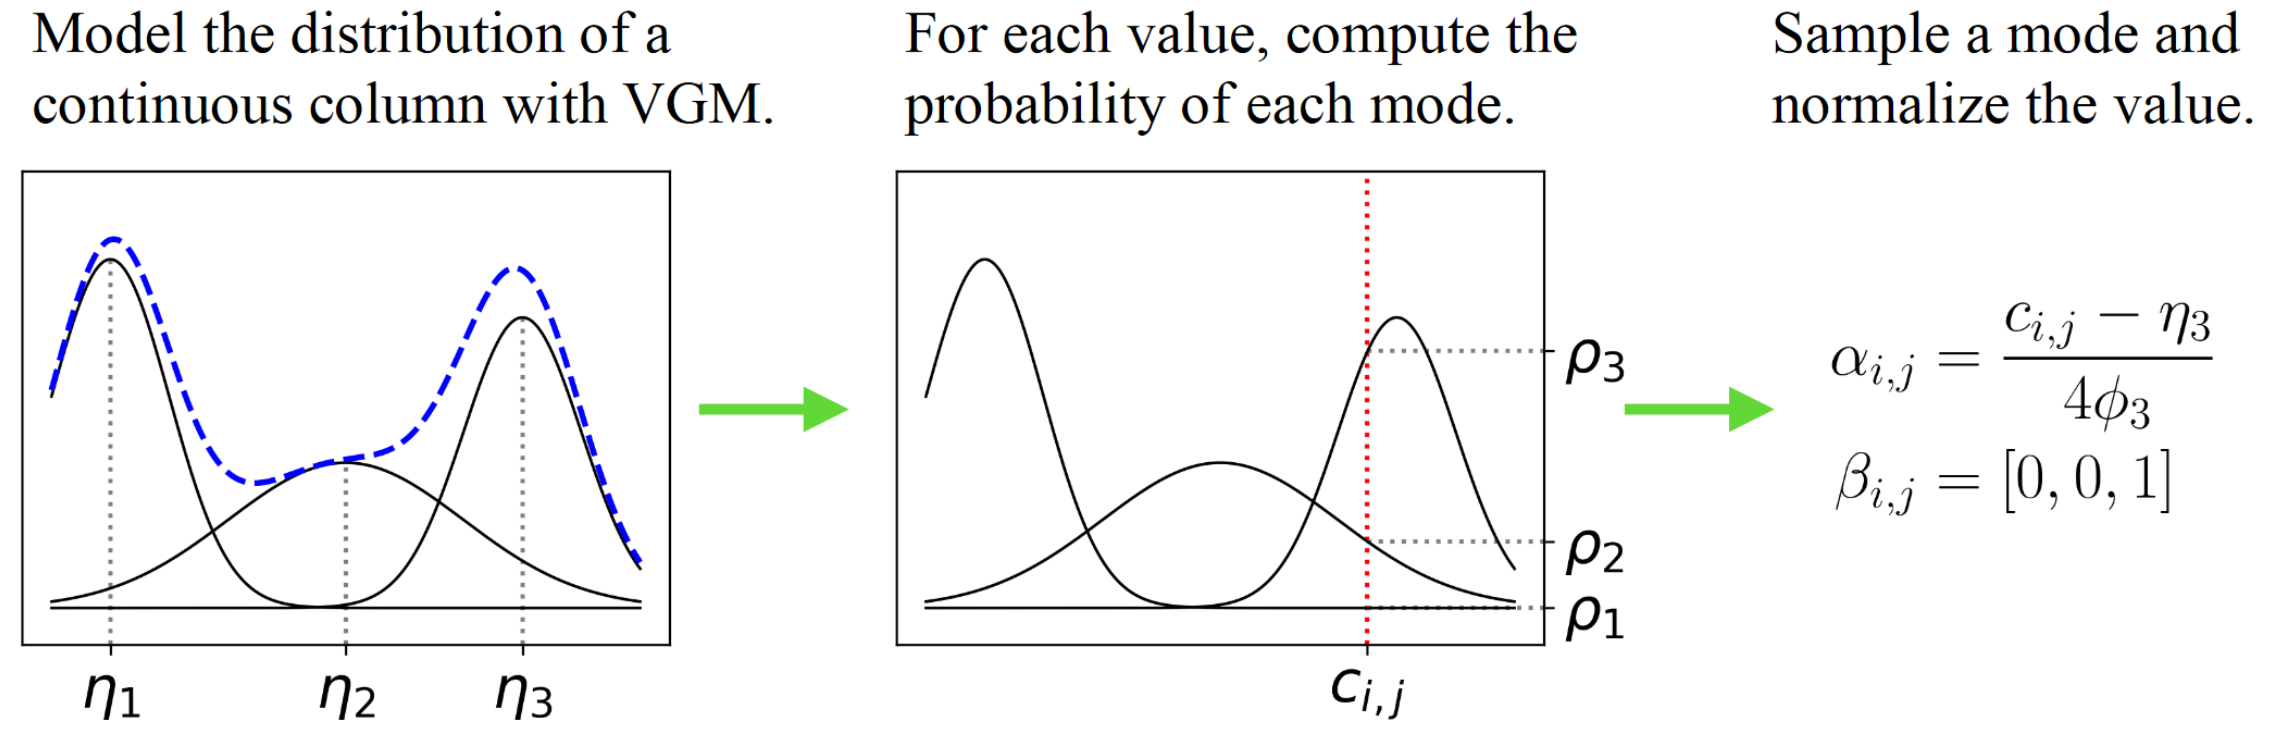
\includegraphics[width=0.8\textwidth]{images/mode-normalization.png}
    \caption[Mode-Specific Normalization]{An example of mode-specific normalization \cite[Figure 1, p. 4]{xu2019ModelingTabularData}}
    \label{fig:mode-specific-normalization}
\end{figure}

Another approach to standardize the range of a column between 0 and 1 is a Quantile-transformation, which is a non-linear transformation \cite{scikit-learndevelopers2023PreprocessingData, kotelnikov2022TabDDPMModellingTabular}.
The Quantile-transformation allows the mapping of all values of a random variable into a desired output distribution, such as the uniform or normal distribution, 
using the quantile function on the inverse cumulative distribution of the random variable. 
This transformation preserves the rank order of the values but distorts correlations and distances within and across features \cite{scikit-learndevelopers2023PreprocessingData}.


%-------------------------------------------------------------------------
\section{Data Synthesis}
\label{ch:preliminaries-dataSynthesis}

\subsection{Synthetic Data}
\label{ch:preliminaries-dataSynthesis-syntheticData}
Synthetic data can be defined as "(...) artificially generated data, that are modeled on real data, with the same structure and properties as the original data (...)" \cite[p. 2]{kaloskampis2020SyntheticDataCivil} 
but without containing any actual specific information or entries of the actual real data. 
While first synthetic data approaches \cite{gelman1992InferenceIterativeSimulation} focused on imputation techniques to generate synthetic data, the advent of deep learning has led to the topic gaining importance \cite{kowalczyk2022TaxonomyUseSynthetic, kaloskampis2020SyntheticDataCivil}.
Acquiring and collecting real data can be costly \cite{panova2022HowSyntheticData} or may simply not be possible due to the sensitivity of the data (\eg medical records) \cite{esteban2017RealvaluedMedicalTimea} or due to regulatory restrictions, such as the \gls{gdpr} \glsadd{gdpraccr} \cite{european_commission_regulation_2016}.
Synthetic data on the other hand is, compared to real data, cheap to generate \cite{leminh2021AirGenGANbasedSynthetica}, fulfils regulatory and privacy constraints \cite{zhao2022CTABGANEnhancingTabular} and can substitute real data in software development for testing \cite{whiting2008CreatingRealisticScenariobased} or machine learning training \cite{panova2022HowSyntheticData}.
Hence, synthetic data could be used as an alternative to real data in various use cases.
Access to data is still one of the biggest bottlenecks when developing machine learning or deep learning models \cite{fan2020RelationalDataSynthesisa}.
Synthetic data could be used to increase the data quality, by rebalancing skewed dataset \cite{zhao2022CTABGANEnhancingTabular} 
or increasing the dataset size as additional training data or in combination with the real data \cite{leminh2021AirGenGANbasedSynthetica, kim2021OCTGANNeuralODEbased}.
Synthetic data can also be used in situations where working with the real data is not possible, due to privacy or availability reasons \cite{9034117, whiting2008CreatingRealisticScenariobased}.
In software development, high-quality test data is crucial for development but challenging and time-consuming to generate \cite{whiting2008CreatingRealisticScenariobased}.
Developers' time to create such datasets is usually scarce and it might be the case that developers do not even have permission to see the data, due to its sensitivity \cite{whiting2008CreatingRealisticScenariobased}.
A synthetic data generation model would possibly allow developers to generate test data with predefined characteristics without it being restricted in any form.


\subsection{Synthetic Tabular Data Generation}
\label{sec: synthetic tabular data generation}

Generative models have recently received a lot of attention, thanks to their impressive results in generating a variety of data formats, 
such as images \cite{ho2020DenoisingDiffusionProbabilistic, dhariwal2021DiffusionModelsBeat, rombach2022HighResolutionImageSynthesis}, videos \cite{ho2022VideoDiffusionModels, runwayGen1Runway}, text \cite{radfordImprovingLanguageUnderstanding, openai2022ChatGPTOptimizingLanguage}, or music \cite{agostinelli2023MusicLMGeneratingMusic, Forsgren_Martiros_2022}.

While synthetic data generation can be applied to various types of data, generating synthetic tabular data is challenging due to the complexity of the underlying joint distributions between variables \cite{borisov2022DeepNeuralNetworks}.
This works formal definition of the tabular data generation is adapted from \cite[p. 2]{xu2019ModelingTabularData} and expands the definition of a table from \autoref{ch:preliminaries-dataSynthesis-tabularData}:

\begin{displayquote}
    A data synthesizer $G$ is trained on a table $T$ and then used to generate a synthetic table $T_{syn}$. % Vllt die definition einer tabelle nach oben packen und von oben übernehmen?
    $T$ is partitioned into a training set $T_{train}$ and test set $T_{test}$. 
    The synthesizer $G$ is trained on $T_{train}$ and afterwards used to sample independently individual rows to create $T_{syn}$.
    Finally, the similarity of $T_{syn}$ to $T_{test}$ is evaluated using a selected similarity evaluation technique.
\end{displayquote}

The synthetic dataset $T_{syn}$ should exhibit a similar relationship with the test dataset partition $T_{test}$ 
as the one found between the training dataset partition $T_{train}$ and $T_{test}$. 
This is crucial for maintaining the underlying structure and properties of the original data.
The primary objective for the generative model $G$ is to create $T_{syn}$ in such a way that it appears to originate from the same joint distribution as the complete dataset $T$. 
This ensures that the synthetic data maintains the essential characteristics of the original data.
Importantly, $T_{syn}$ is not directly compared to $T_{train}$, because the purpose of generating $T_{syn}$ is not to merely replicate $T_{train}$,
but to create a new dataset that preserves the inherent relationships and properties of the original data.

During the generation of synthetic tabular data, there are two competing objectives: high data utility and low disclosure risk.
Data utility is concerned with how well the synthetic data accurately reflects the real data in terms of its underlying patterns and relationships.
Low disclosure risk on the other hand is concerned with the preservation of privacy and confidentiality of the information in the real training dataset $T_{train}$ \cite{little2021GenerativeAdversarialNetworksa}. 

Tabular data synthesis approaches can be divided into process- and data-driven methods \cite{goncalves2020GenerationEvaluationSynthetic}.
Process-driven models focus on simulating real-world processes and gather data during that simulation to create the synthetic dataset \cite{goncalves2020GenerationEvaluationSynthetic, kowalczyk2022TaxonomyUseSynthetic}.
On the other hand, data-driven approaches aim to generate synthetic data based on already existing real-world datasets \cite{goncalves2020GenerationEvaluationSynthetic, kowalczyk2022TaxonomyUseSynthetic}.
This can be achieved by augmenting the existing dataset, \ie applying transformations to the existing individual datapoints to generate new datapoints \cite{kowalczyk2022TaxonomyUseSynthetic}.
Another technique to generate synthetic data is to simply sample from the individual feature distributions of a dataset to create new synthetic data \cite{kowalczyk2022TaxonomyUseSynthetic}.
Lastly, machine learning and deep learning algorithms can be used to learn the underlying joint distributions of the real data to generate new synthetic data \cite{kowalczyk2022TaxonomyUseSynthetic}. 
%challanges
Compared to other data types, the synthesis of tabular data is especially challenging due to its heterogeneity, potential weak correlations among features and the dependency on preprocessing \cite{borisov2022DeepNeuralNetworks, yoon2020VIMEExtendingSuccess, gorishniy2022EmbeddingsNumericalFeatures}.
To create a realistic synthetic dataset, interdependencies that may exist between variables must be captured and 
it is possible that the model overfits on the training data and generalizes relationships between features that are only present in training but not in the test data \cite{lederrey2022DATGANIntegratingExperta}.
In addition to that, tabular data columns can follow complex distributions, which makes the synthesis challenging.
\textcite{zhao2022CTABGANEnhancingTabular} identified the following four properties of tabular data, one should consider when trying to synthesize tabular data:

\begin{enumerate}
    \item \textbf{Single Gaussian variables}: Data where its distribution follows a Gaussian distribution \cite{zhao2022CTABGANEnhancingTabular}.
    \item \textbf{Mixed data type variables}: A single column can contain a mix of continuous and categorical values. 
    For instance, a \textit{Loan} column could hold information about the size of an individual's loan.
    The values in this column are mostly positive float values but can also take the value \textit{$-1$} which indicates that this person did not get approved for a loan.
    Such a special categorical value in an otherwise purely numerical column needs to be considered when working with this column \cite{zhao2022CTABGANEnhancingTabular}.
    \item \textbf{Long tail distributions}: In real-world data, most data points may occur "near the initial value of a distribution and rare cases towards the end" \cite[p. 3]{zhao2022CTABGANEnhancingTabular}.
    This results in a tail-like distribution.
    The phenomenon of long-tail distribution is seen across a variety of applications including object detection, scene parsing, document processing, and item recommendation \cite{zhou2018DeepSuperclassLearning}.
    Capturing these long-tail distributions correctly during the synthesis is important, not only because they represent unique or rare scenarios that could be crucial for certain analysis tasks, but also because the minority classes in the tail collectively constitute a significant portion of the entire dataset \cite{zhou2018DeepSuperclassLearning}. 
    \item \textbf{Skewed multi-mode continuous variables}: Complex numerical distributions do not necessarily follow a single Gaussian distribution.
    It is possible for their distribution to consist of multiple unknown distributions that are potentially skewed as well. 
    Their conjunction as a whole makes up the complex distribution \cite{zhao2022CTABGANEnhancingTabular}, as it could be seen in the example of \autoref{fig:mode-specific-normalization}.
\end{enumerate}

A successful tabular data generator should be able to recreate such properties of real data in their synthetic data counterpart.


\section{Deep Learning Architectures}
\label{ch:preliminaries-deepLearningArchitectures}

Deep learning has rapidly become a dominant force in artificial intelligence, revolutionizing various fields including computer vision, \gls{nlp}, and generative modeling. 
Here, complex neural networks architectures emerged with multiple layers and complex interconnections.
These architectures have enabled the creation of highly accurate and efficient models that are capable of processing vast amounts of data from different modalities.

In recent years, this development of new deep-learning architectures has been a key area of research, leading to the creation of such powerful models.
This section will start with a high-level introduction into a neural network's most important architectural building blocks.
Afterwards, the most important deep learning model architectures for generating data are presented.

\subsection{Neural Networks}
\label{ch:preliminaries-deepLearningArchitectures-neuralNetworks}

The most basic neural network is called a perceptron \autoref{fig:perceptron} \cite{rosenblatt1958PerceptronProbabilisticModel}.
It consists of a single input layer that is connected to an output node.
Each input node is connected with the output node via weight edges.
For all inputs, the input value is multiplied by each respective weight.
The sum of all input-weights' multiplication serves as the input to an activation function, which is different depending on the task at hand.
The output is the prediction of the perceptron which is compared to the actual result, the label, and an error is calculated.
This error is later used to update the individual nodes' weights via backpropagation \cite{aggarwal2018NeuralNetworksDeep}.
The output of one node can also serve as the input to another node, so multiple layers of nodes are created.
This is referred to as a \gls{mlp} or feed-forward neural network as presented in \autoref{fig:mlp}, 
because the information flows forward from input through the multiple layers in the middle (also called hidden layers) to the output \cite{aggarwal2018NeuralNetworksDeep, Goodfellow-et-al-2016}.
An \gls{mlp} tries to approximate some function $f^*$ by defining a mapping $y=f(x;\theta)$ and learning the values of the parameters $\theta$ (\ie the weights) that best approximate $f^*$ \cite{Goodfellow-et-al-2016}.
A simple \gls{mlp} is already able to learn almost any function, which is why they are also considered to be universal function approximators \cite{aggarwal2018NeuralNetworksDeep, hornik1989MultilayerFeedforwardNetworks}.


\begin{figure}
    \begin{subfigure}{0.8\textwidth}
      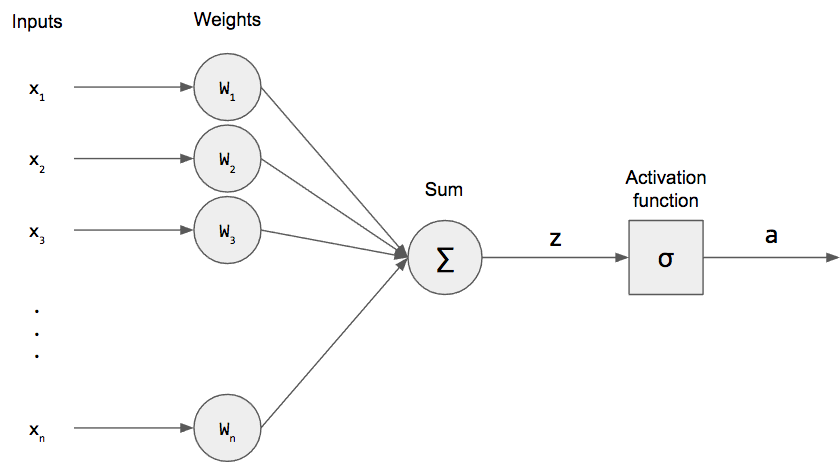
\includegraphics[width=\linewidth]{images/perceptron.png}
      \caption[Perceptron]{Perceptron} \label{fig:perceptron}
    \end{subfigure}%
    \hspace*{\fill}   % maximize separation between the subfigures
    \begin{subfigure}{0.8\textwidth}
      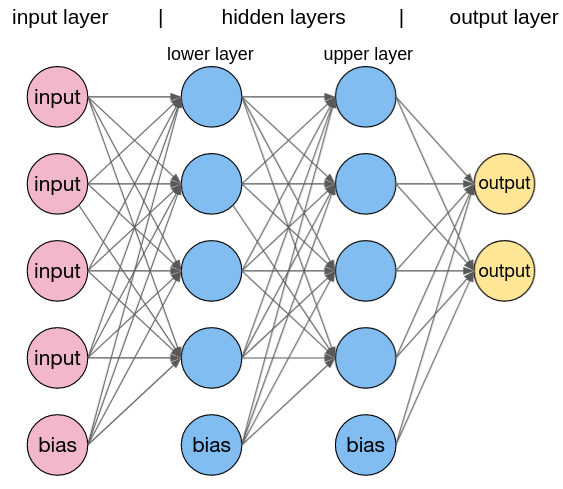
\includegraphics[width=\linewidth]{images/mlp.png}
      \caption[Multilayer Perceptron]{multilayer perceptron} \label{fig:mlp}
    \end{subfigure}%
    \hspace*{\fill}   % maximizeseparation between the subfigures
  \caption[Overview Perceptron]{Overview Perceptron} \label{fig:NN_Overview}
\end{figure}

Convolutional networks, or \glspl{cnn} \cite{lecun1998GradientbasedLearningApplied}, are a specialized type of neural network.
As their name indicates, they perform convolutions on the data as illustrated in \autoref{fig:cnns}.
Convolution can be defined as "a dot-product operation between a grid-structured set of weights and similar grid-structured inputs drawn from
different spatial localities in the input volume" \cite[p. 316]{aggarwal2018NeuralNetworksDeep}.
In other words, a small grid of numbers called \textit{weights} slides over a larger grid of numbers, which is in the context of deep learning usually an image.
In each position, the numbers in the small grid are multiplied by the corresponding numbers they cover in the large grid, and these results are added together. 
This process is repeated across different areas by sliding the small grid over the large grid repeatedly until the complete large grid was processed.
The weights within the small grid, often referred to as the \textit{kernel}, get adjusted during training of the \gls{cnn} during backpropagation. 
This fine-tunes these weights based on how far off the network's output is from the expected output, enabling the convolutional network to improve its performance over time \cite{aggarwal2018NeuralNetworksDeep, Goodfellow-et-al-2016}.

\glspl{cnn} perform exceptionally well on data with a grid-like topology with strong spatial dependencies such as image or time-series data \cite{aggarwal2018NeuralNetworksDeep, Goodfellow-et-al-2016}.
In a typical convolutional network, a layer starts by performing multiple convolution operations in parallel on the data.
The linear activations that are produced by the convolutions are sent through a non-linear activation function (usually a \gls{relu}).
Lastly, a pooling function is applied to the output of the activation function \cite{aggarwal2018NeuralNetworksDeep}.
A pooling function reduces the spatial size of the created feature maps while retaining their essential features \cite{Goodfellow-et-al-2016, aggarwal2018NeuralNetworksDeep}.
\textcite[p. 335]{Goodfellow-et-al-2016} also describe it as a type of "summary statistic of the nearby outputs".
Pooling allows the features extracted by the \gls{cnn} to be less sensitive to changes in the position of the input data.
This property is known as translation invariance and is one of the reasons why \glspl{cnn} perform so well with data formats that have local spatial dependencies \cite{Goodfellow-et-al-2016, aggarwal2018NeuralNetworksDeep}.
Another way to reduce the dimensionality is to increase the convolution stride.
A stride refers to the step size or the number of pixels by which the filter, also known as the convolutional kernel, moves across the input feature map during the convolution operation \cite{aggarwal2018NeuralNetworksDeep}.
The effect of using a stride greater than 1 is that it reduces the spatial dimensions of the output feature map. 
Specifically, the height and width of the output are determined by the formula $(L_q - F_q)/S_q + 1$, where $L_q$ is the height (or width) of the input, $F_q$ is the size of the filter, and $S_q$ is the stride in layer $q$ \cite[p. 324]{aggarwal2018NeuralNetworksDeep}.

In feed-forward neural networks, information flows forward through the network from input to output node, hence, there are no internal connections that allow
the output of the model to be fed back into the network as inputs \cite{aggarwal2018NeuralNetworksDeep, Goodfellow-et-al-2016}.
When such connections are added to the network architecture, the resulting models are referred to as \glspl{rnn} \cite{rumelhart1986LearningRepresentationsBackpropagating}.
\Glspl{rnn} are designed to process sequential data, like sentences or time-series data, where the size of the sequence does not have to be fixed.
In \glspl{cnn}, the learned parameters are shared by using the same convolution kernel on each subset of neighbouring input data at each time step (\autoref{fig:rnns}). 
As a result, a succession of output values is produced, each of which is dependent on a few close input values. 
\glspl{rnn} share parameters differently since each output value depends on its predecessors' output. 
This enables parameter sharing via a deep computational graph by allowing the same update algorithm to be applied to all outputs.
When processing a sequence, \eg a sentence, a \gls{rnn} receives one datapoint, \eg a word, at each timestep.
The network itself has a so-called \textit{hidden state} that is kept throughout all timesteps and changes with each timestep.
This, however, means that the output $y_3$ of the input at $x_{t=3}$ depends on the hidden states $h_0$ through $h_3$ and input $x_0$ through $x_3$.
As a result, the computational graph on which the backpropagation is performed on increases as well \cite{aggarwal2018NeuralNetworksDeep}.
A large computation graph introduces new practical issues, such as an increased computation time and during the training, helpful information might not be propagated from output to the end of the model,
due to the vanishing and exploding gradient phenomenon \cite{aggarwal2018NeuralNetworksDeep}.
To address these issues, further improvements to the architecture have been made, such as \glspl{lstm} \cite{hochreiter1997LongShortTermMemory} or \glspl{gru} \cite{cho2014PropertiesNeuralMachine}.

Over time, additional architectural design choices have been discovered that have led to further improvements and solved other issues that emerged during the development of neural networks.
One such design is the ResNet \cite{he2016DeepResidualLearning} which introduced residual connections between layers as depicted in \autoref{fig:resnet} \cite{he2016DeepResidualLearning, aggarwal2018NeuralNetworksDeep}.
The connections, also called skip connections, allow information to be copied over layers and allow the backpropagated gradient information to skip specific layers, if necessary \cite{he2016DeepResidualLearning, aggarwal2018NeuralNetworksDeep}.
This is achieved by adding the output of one layer directly to the output of a later layer, bypassing one or more intermediate layers.
This way, even a very small gradient can flow more easily back through the network during backpropagation of the gradient, alleviating the vanishing gradient problem and enabling better learning capabilities \cite{he2016DeepResidualLearning, aggarwal2018NeuralNetworksDeep}.
The decision of which layers to skip is learned by the model itself during the training through the backpropagation algorithm \cite{he2016DeepResidualLearning, aggarwal2018NeuralNetworksDeep}.

\begin{figure}
    \begin{subfigure}{0.7\textwidth}
      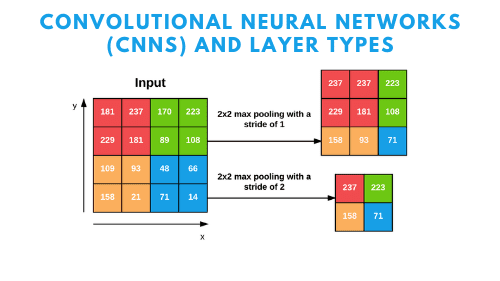
\includegraphics[width=\linewidth]{images/cnns.png}
      \captionsetup{justification=centering}
      \caption{Convolution \\(adapted from \cite{rosebrock2021ConvolutionalNeuralNetworks})} \label{fig:cnns}
    \end{subfigure}%
    \hspace*{\fill}   % maximize separation between the subfigures
    \begin{subfigure}{0.7\textwidth}
      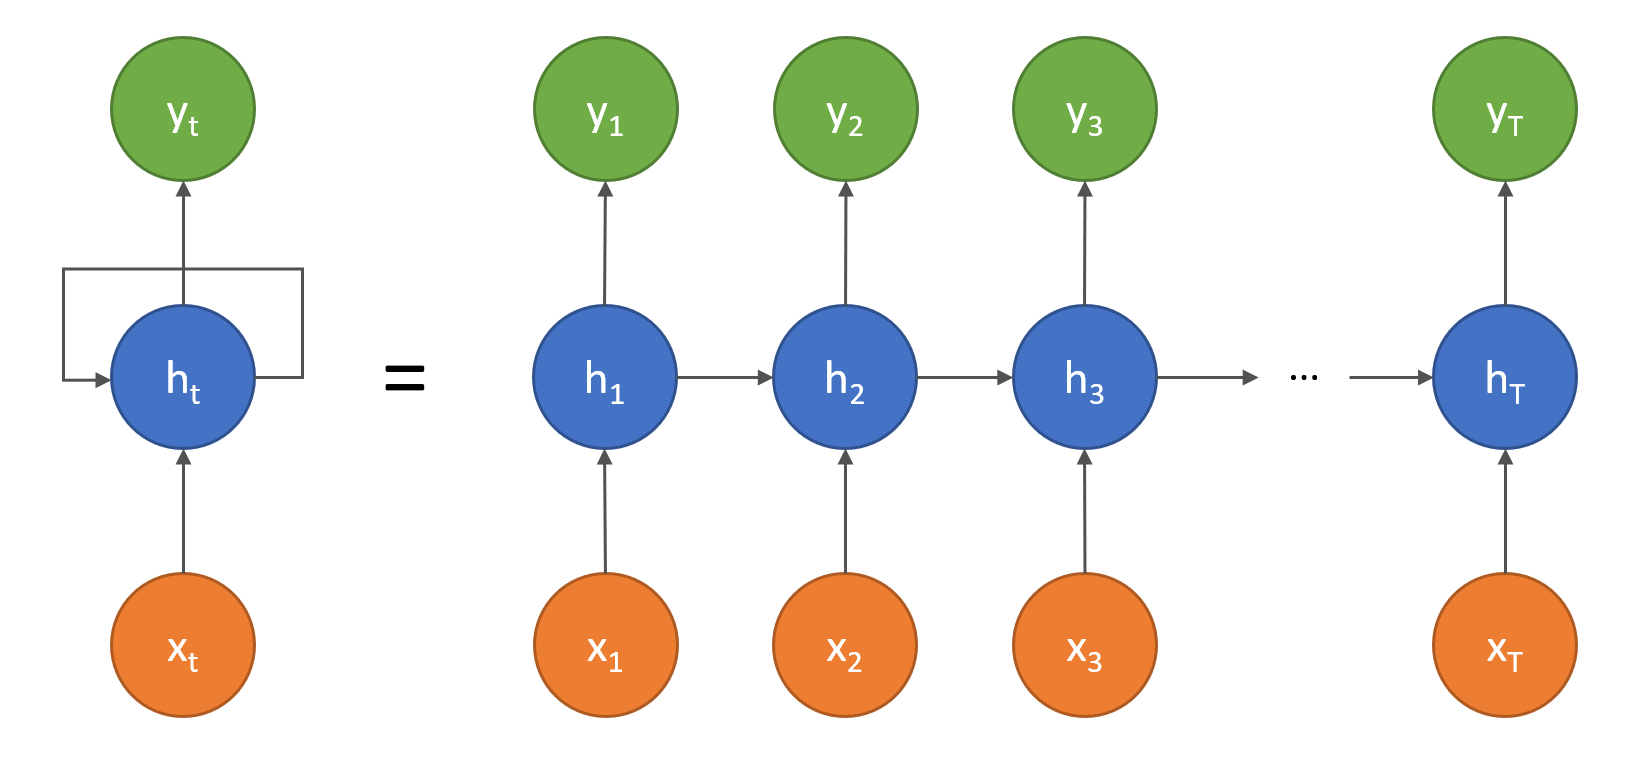
\includegraphics[width=\linewidth]{images/rnns.png}
      \captionsetup{justification=centering}
      \caption{\Gls{rnn} \\(adapted from \cite{radhakrishnan2017IntroductionRecurrentNeural})} \label{fig:rnns}
    \end{subfigure}%
    \hspace*{\fill}   % maximizeseparation between the subfigures
    \begin{subfigure}{0.7\textwidth}
        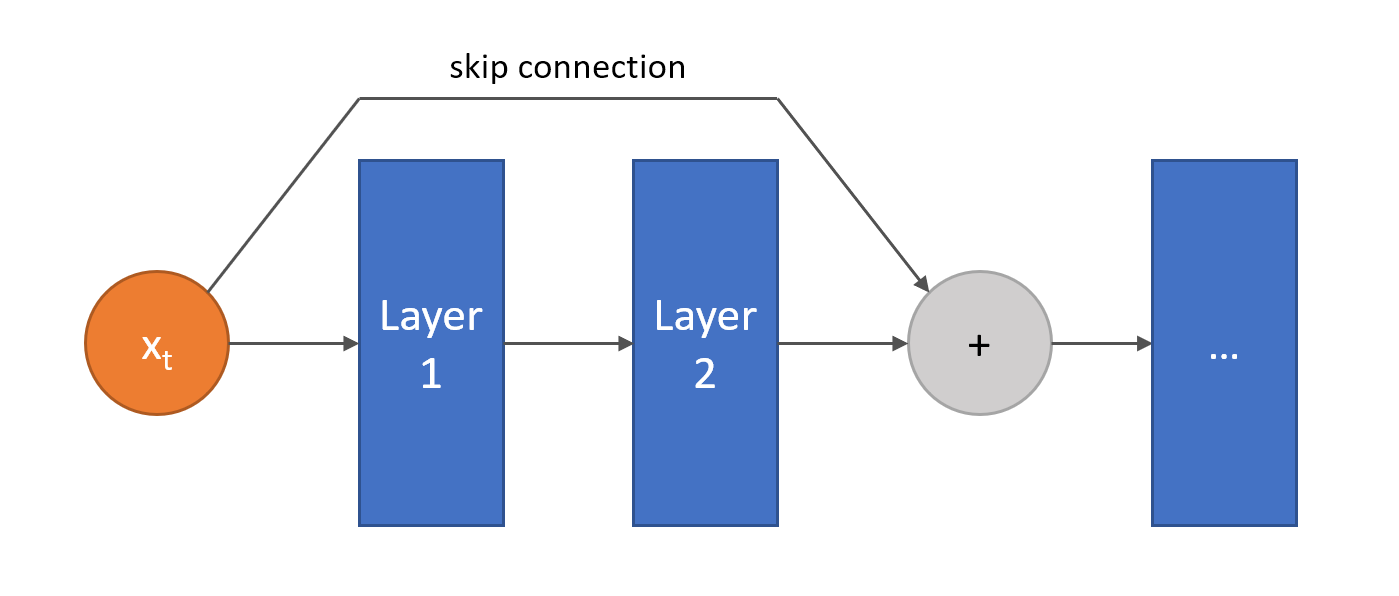
\includegraphics[width=\linewidth]{images/resnet.png}
        \captionsetup{justification=centering}
        \caption{Residual Connection \\(adapted from \cite{hassan2019ResNet3450})} \label{fig:resnet}
      \end{subfigure}%
    \hspace*{\fill}   % maximizeseparation between the subfigures
  \caption[Overview Neural Network Architectures]{Overview Neural Network Architectures} \label{fig:NN_architectures_Overview}
\end{figure}

Lastly, inspired by the human cognitive capabilities to focus on specific parts of an input, attention mechanisms have been introduced \cite{niu2021ReviewAttentionMechanism, aggarwal2018NeuralNetworksDeep}.
The implementation of attention in neural networks tries to address the problem of information overload and is supposed to enable the network to allocate its resources \cite{niu2021ReviewAttentionMechanism}.
Information overload in the context of deep learning typically refers to issues that arise when a model is fed with too much data, that can hinder the model to capture the relevant information.
Issues during training may arise if the input data contains too much noise, that is of no relevance or might cause the model to rather learn to predict the noise, than the actual target.
With this, the model may overfit the training data and perform poorly on the test data. 
An attention mechanism has been successfully applied to various tasks in different domains, such as computer vision or \gls{nlp} \cite{niu2021ReviewAttentionMechanism}.
The architectural realization of attention is realized differently, depending on the task at hand \cite{aggarwal2018NeuralNetworksDeep}.
The attention mechanism in computer vision involves weighting different regions of the image based on their relevance to the task \cite{aggarwal2018NeuralNetworksDeep}. 
This can be achieved through techniques such as spatial attention, channel attention or temporal attention \cite{guo2022AttentionMechanismsComputer}.
In \gls{nlp}, attention mechanisms try to improve to capture the meaning of a sentence \cite{niu2021ReviewAttentionMechanism}. 
For instance, this has been achieved through the introduction of a context vector in an \gls{rnn} encoder-decoder \cite{DBLP:journals/corr/BahdanauCB14} or through self-attention \cite{vaswani2017AttentionAllYou} (see \autoref{ch:preliminaries-transformers} for a detailed explanation of self-attention).

\section{Deep Generative Models}
\label{ch:preliminaries-generativeMlgorithms}

Deep generative models have revolutionized the field of artificial intelligence and machine learning by generating new and original data based on existing patterns and structures. 
Generative models try to learn a joint distribution over all the available variables in a dataset \cite{kingma2019IntroductionVariationalAutoencoders}, which is also called the \textit{generative modeling problem} \cite{goodfellow2020GenerativeAdversarialNetworks}.
Formally, in generative modeling training examples $x$ are drawn from an unknown distribution $p_{data}(x)$ and a generative modeling algorithm is trained to learn a distribution density function $p_{model}(x;\theta)$ that approximates the true probability density function $p_{data}(x)$ as closely as possible \cite[p. 139]{goodfellow2020GenerativeAdversarialNetworks}.
$\theta$ are the models parameters that determine the models output, they are usually learned by searching for best $\theta$ values that result in $p_{model}$ to be as similar to $p_{data}$ as possible \cite[p. 139]{goodfellow2020GenerativeAdversarialNetworks}.

Several powerful generative modeling approaches with different architectures have emerged, each with its strengths and weaknesses. 
This section will explore four of the most popular approaches: \glspl{vae} (\autoref{ch:preliminaries-variationalAutoencoders}), \glspl{gan} (\autoref{ch:preliminaries-generativeAdversarialNetworks}), transformers (\autoref{ch:preliminaries-transformers}), and diffusion models (\autoref{ch:preliminaries-diffusionProbabilisticModels}). 

\subsection{Variational Autoencoders}
\label{ch:preliminaries-variationalAutoencoders} 

In order to understand \glspl{vae} \cite{kingma2013AutoEncodingVariationalBayes}, an introduction to vanilla autoencoders is required.
Autoencoders, firstly introduced in \cite{rumelhart1986LearningInternalRepresentations}, are a neural network architecture designed to generate a copy of the input \cite{Goodfellow-et-al-2016, Bank2020Autoencoders}.
This is done by compressing the original input $x$ into a meaningful representation by constricting the number of nodes in the intermediate hidden layer \cite{aggarwal2018NeuralNetworksDeep, Bank2020Autoencoders}, also called bottleneck.
\autoref{fig:ae} shows that an autoencoder consists of two deep-learning modules, the encoder, and the decoder.
The encoder function (or generative model \cite{kingma2019IntroductionVariationalAutoencoders}), $z=g(x)$ receives an input $x$ and creates a latent representation $z$ (also called "code" \cite{aggarwal2018NeuralNetworksDeep}) with a dimensionality smaller than $x$ \cite{Goodfellow-et-al-2016, Bank2020Autoencoders}.
The decoder (or recognition model \cite{kingma2019IntroductionVariationalAutoencoders}) receives the latent representation $z$ and tries to reconstruct the original input, $r=f(z)$ with the same dimensionality as $x$ \cite{Goodfellow-et-al-2016}.
The reconstruction of the input $x$, designated as $r$, is also commonly referred to as $x'$. 
The objective is to ensure that $x'$ is as similar as possible to the original input $x$.
For the autoencoder to learn and optimize the model's parameters, a loss $L$ is calculated by applying a reconstruction loss function, which measures how close the reconstruction is to its original counterpart \cite{Bank2020Autoencoders, maheshwari2022AutoencoderIssuesChallenges}.
The reconstruction loss depends on the use case, for instance, it could be the Mean-squared error between $x$ and $r$, $L=\sum_{i=1}^{N}(x_i-r_i)^2$ for $N$ features in $x$, \cite{aggarwal2018NeuralNetworksDeep, Goodfellow-et-al-2016}.
Since $z$ is restricted in dimensionality, a simple copying from input to output, \ie $f(g(x))=x$, should not be possible, and the encoder should learn to create an approximation of $x$ with its most essential features \cite{aggarwal2018NeuralNetworksDeep}.
Therefore, autoencoders are a dimensionality reduction technique.
The latent representation of a complete linear autoencoder without any non-linear operations achieves the same representation as a \gls{pca} \cite{plaut2018PrincipalSubspacesPrincipal, Bank2020Autoencoders}.
Further variations of autoencoders have emerged.
Deep autoencoders expand the neural network from one hidden layer to multiple layers with non-linear activation functions, increasing the representation power \cite{aggarwal2018NeuralNetworksDeep}.
Other variants include denoising autoencoders, convolutional autoencoders, or sparse autoencoders \cite{maheshwari2022AutoencoderIssuesChallenges, Goodfellow-et-al-2016}.
However, vanilla autoencoders lack regularity in the latent space which means they struggle with interpolation for datapoints that have not been present in the input sequence \cite{razghandi2022VariationalAutoencoderGenerativea}.




\glspl{vae} increase the reconstruction robustness by letting the decoder sample from continuous distributions \cite{kingma2013AutoEncodingVariationalBayes}.
% \glspl{vae} are, as the name suggests, making use of stochastic variational inference, where the goal is to approximate complex distributions (like the posterior) by simpler ones (like the Gaussian distribution in this case), enabling efficient computation and handling of uncertainty.
This is achieved by introducing the \gls{kl} divergence (see \autoref{eqn:kl-divergence}) to ensure that the latent space representation follows a standard Gaussian distribution (zero mean and unit variance) \cite{razghandi2022VariationalAutoencoderGenerativea, aggarwal2018NeuralNetworksDeep}.
Instead of the encoder mapping the input into a fixed vector $z$, it is mapped into a distribution by generating two vectors representing the mean $\mu$ and standard deviation $\sigma$ of the distribution (see \autoref{fig:vae}) \cite{razghandi2022VariationalAutoencoderGenerativea, aggarwal2018NeuralNetworksDeep}.
Constraining the hidden representation $z$ to a Gaussian distribution allows the decoder to generate new data by simply feeding samples from the standard normal distribution \cite{aggarwal2018NeuralNetworksDeep}.
However, if every object is generated from the same distribution, distinguishing between different objects or reconstructing them from a given input would be impossible.
Thus, the distribution of the encoded information $z$, conditioned on a specific input $x$, would differ from the standard normal distribution \cite{aggarwal2018NeuralNetworksDeep}. %p. 207
Hence, the constraint that the hidden representation $z$ follows a standard normal distribution would not be achieved across the encoded distribution from a single object but rather for the entire dataset \cite{aggarwal2018NeuralNetworksDeep}.
The encoder is represented as $q(z|x)$, creating the conditional distribution from which the latent vector is sampled $z\sim q(z|x)$ \cite{kingma2013AutoEncodingVariationalBayes}.
However, this stochastic sampling process makes computations non-differentiable.
In other words, the backpropagation of the gradient is not possible and our neural networks weights cannot be updated \cite{aggarwal2018NeuralNetworksDeep}.
To address this issue, a "reparameterization trick (\autoref{eqn:reparameterization}) was introduced \cite[p. 4]{kingma2013AutoEncodingVariationalBayes}.
Since $z$ is normally distributed ($z\sim N(\mu,\sigma^2)$) it can be rewritten as $z=\mu+\sigma\epsilon$ with $\epsilon$ used as an auxiliary noise variable $\epsilon \sim N(0,1)$ sampled from the standard normal distribution \cite{kingma2013AutoEncodingVariationalBayes}.

\begin{equation}
  \label{eqn:reparameterization}
  N(\mu,\sigma^2) =\mu+\sigma\epsilon
\end{equation}


This transformation moves the stochastic sampling process to the fixed $\epsilon$ variable. 
It allows $\mu$ and $\sigma$ to be differentiable variables, which enables the gradient to flow and the neural network to learn \cite{kingma2013AutoEncodingVariationalBayes}.
In order for the model to learn that $z$ should be close to a normal distribution, a regularization loss is introduced using the \gls{kl}-divergence.
The \gls{kl}-divergence is defined as:

\begin{equation}
    \label{eqn:kl-divergence}
    KL(p\parallel q) = \sum_{i}^{N}p_i\cdot log(\frac{p_i}{q_i})
\end{equation}

with distributions $p$ and $q$:

\begin{equation}
    \label{eqn:regularization_loss}
    L_{regularization} = KL(q(z|x) \parallel p(z))
\end{equation}

The \gls{kl}-divergence measures how diverged two probability distributions are from one another.
With $p(z)$ as a prior defined standard Gaussian distribution, minimizing this function means optimizing the encoders ($q(z|x)$) parameters of $\mu$ and $\sigma$ towards resembling the distributions it is compared to.

Additionally, a reconstruction loss is computed based on the negative log-likelihood that measures the error between the input and output:
% This reconstruction loss is minimized:
\begin{equation}
    \label{eqn:reconstruction_loss}
    L_{reconstruction} =-\mathbb{E}_{q(z|x)}[logp(x|z)]
\end{equation}
with $E_{q(z|x)}$ denoting the expectation with respect to the encoder distribution.

Hence, the final loss function that is minimized during the training of the \gls{vae} is the combination both loss functions\footnote{The loss components in the original work \cite{kingma2013AutoEncodingVariationalBayes} are formulated as a maximization objective. In practice, a loss that can be minimized during training is required. Hence, we convert the maximization objective to a minimization objective by multiplying it with -1}:

\begin{equation}
    \label{eqn:vae_loss}
    L_{vae} =\mathbb{E}_{q(z|x)}[logp(x|z)]-KL(q(z|x) \parallel p(z))
\end{equation}


\begin{figure}[H]
  \centering
  \begin{subfigure}{0.8\textwidth}
    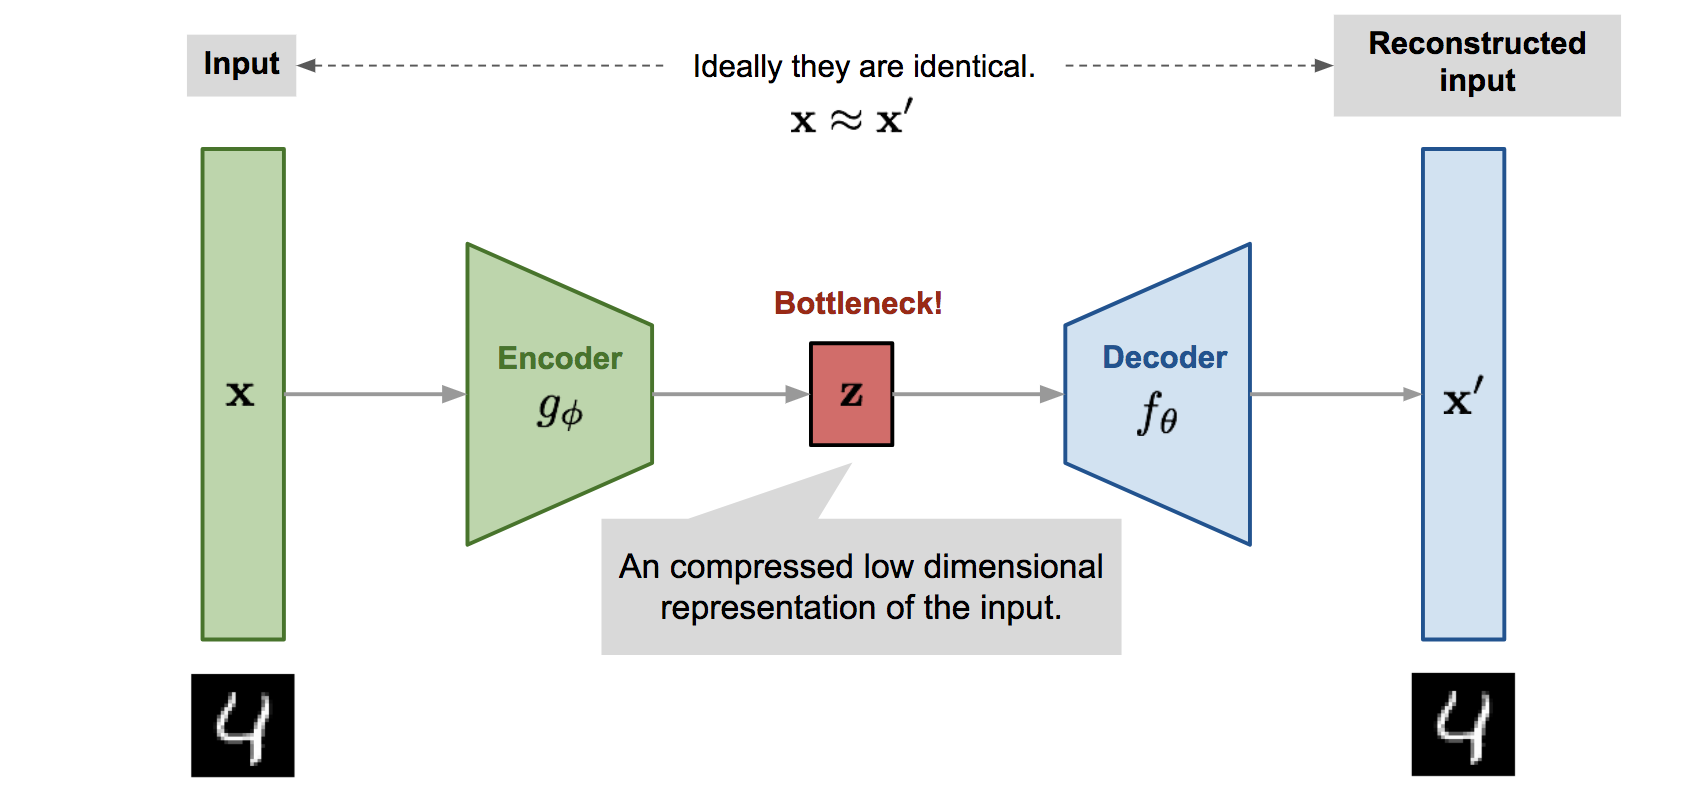
\includegraphics[width=\linewidth]{images/ae.png}
    \caption{Autoencoder} \label{fig:ae}
  \end{subfigure}
  \vspace{\baselineskip}   % separation between the subfigures
  \begin{subfigure}{0.8\textwidth}
    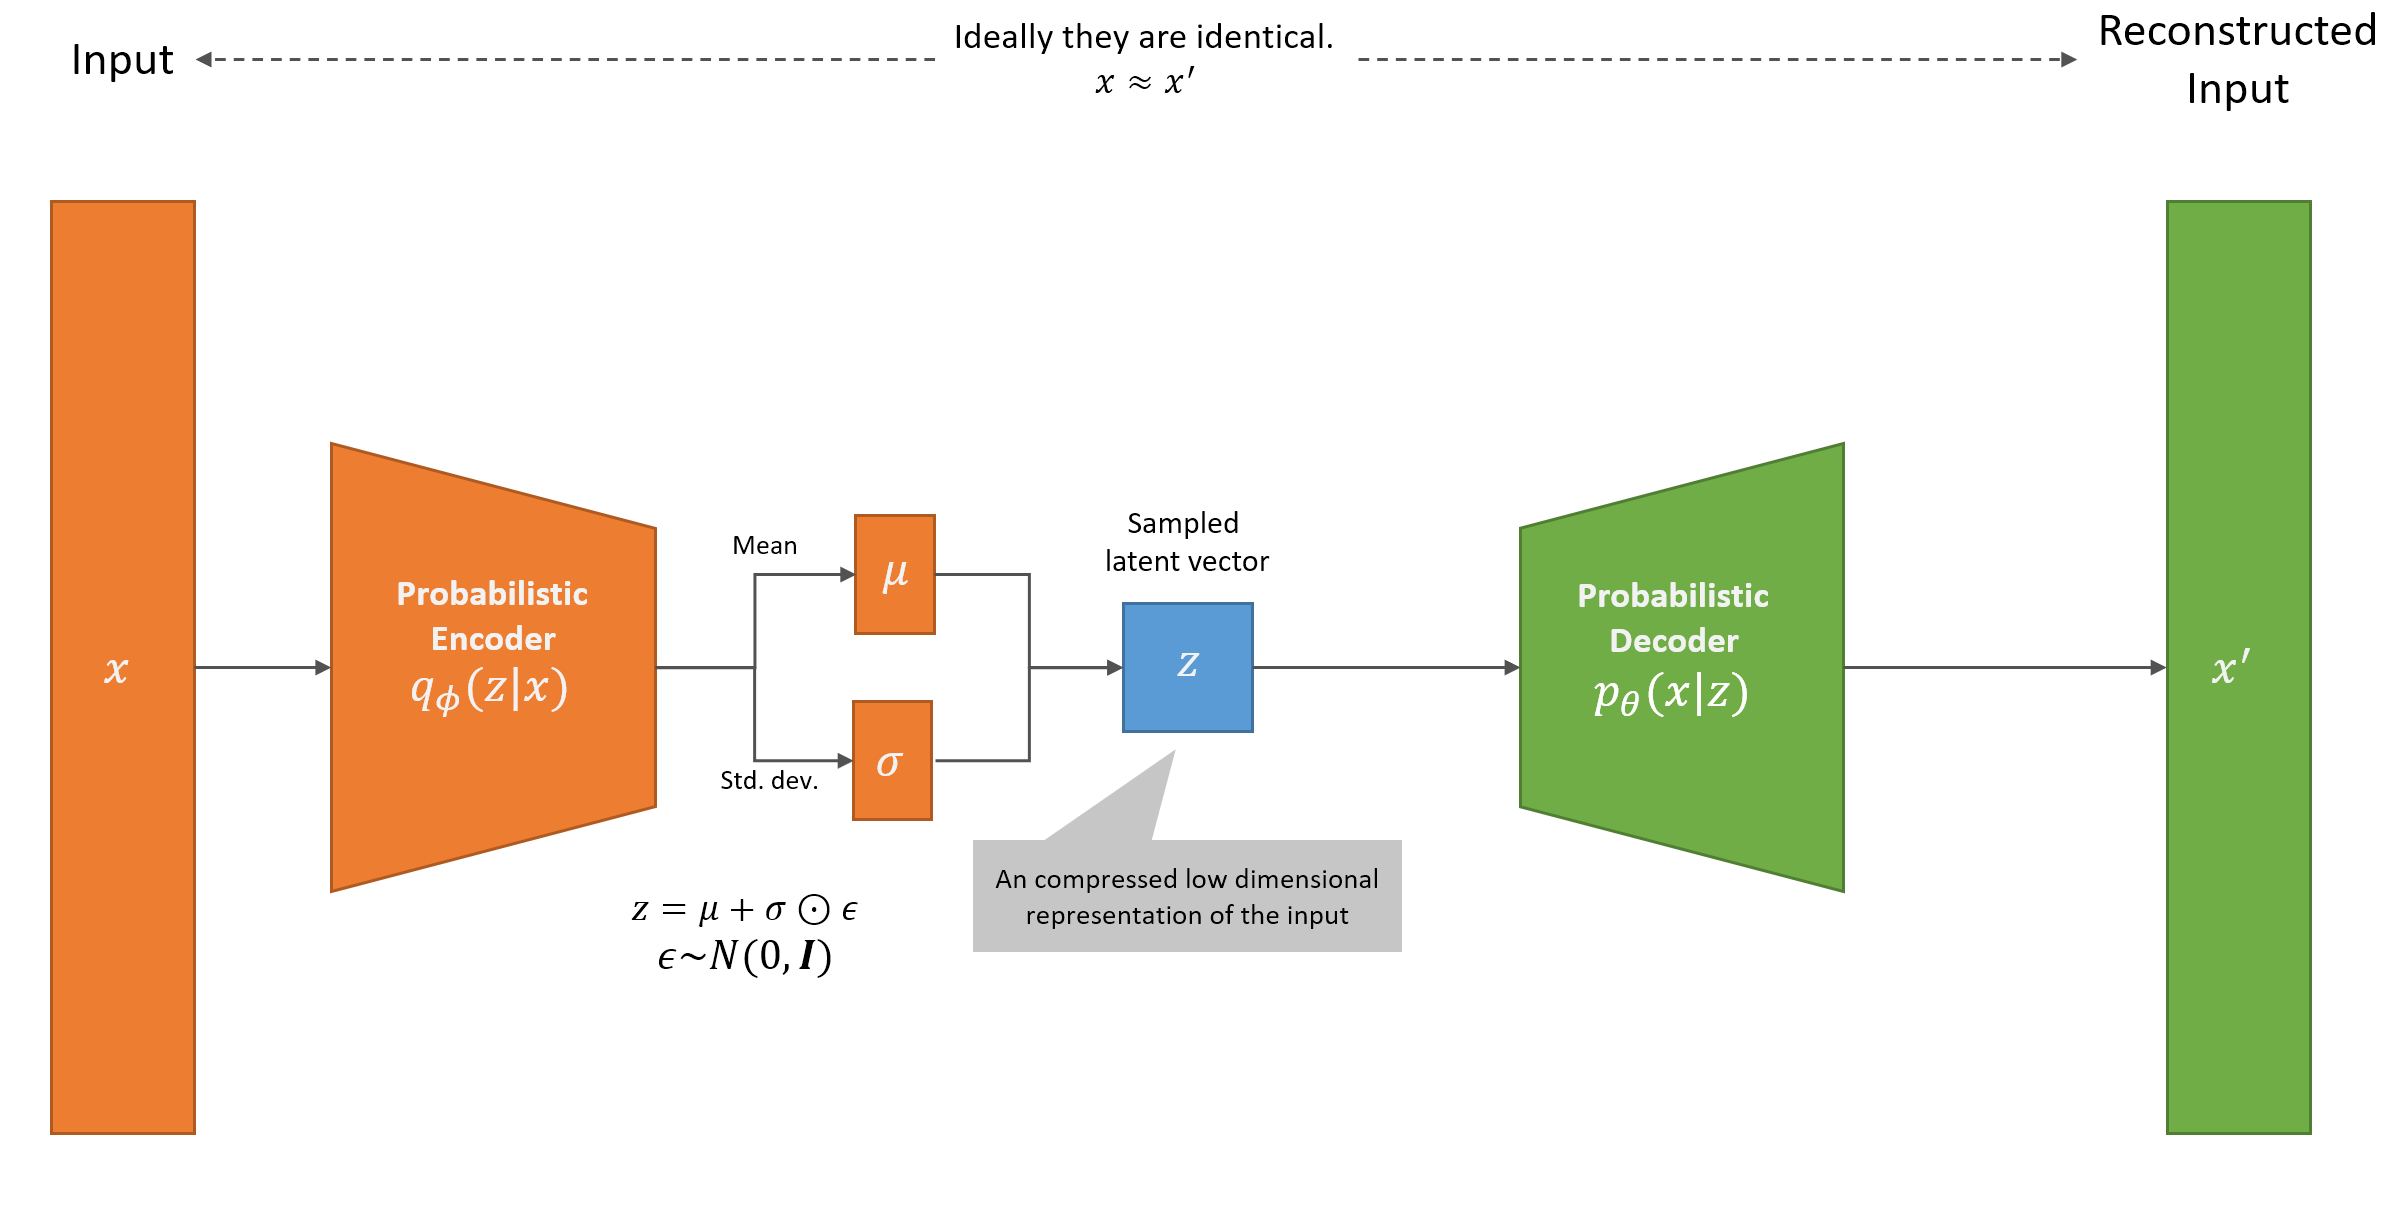
\includegraphics[width=\linewidth]{images/vae.png}
    \caption{Variational Autoencoder} \label{fig:vae}
  \end{subfigure}
\captionsetup{justification=centering}
\caption[Autoencoders]{Architecture of Autoencoder and Variational Autoencoder (adapted from \cite{weng2018AutoencoderBetaVAE})} \label{fig:vae_overview}
\end{figure}



\subsection{Generative Adversarial Networks}
\label{ch:preliminaries-generativeAdversarialNetworks}

\Glspl{gan} \cite{NIPS2014_5ca3e9b1} have been introduced in 2014 as a new architecture to address the generative modeling problem.
The architecture of \glspl{gan} is based on game theory where two models compete in a zero-sum min-max game \cite{NIPS2014_5ca3e9b1, zhao2022CTABGANEnhancingTabular}.
A zero-sum min-max game, in the \glspl{gan}, refers to the adversarial interaction between two models - the generator and the discriminator - where one model's gain (minimizing its loss) corresponds to the other model's loss (maximizing its loss), such that the total sum of their gains and losses is always zero.
While the generator is tasked to generate realistic-looking data points, its adversary, the discriminator is tasked to discriminate whether a given datapoint is a real datapoint or a fake datapoint produced by the generator.
The generator function $G(z;\theta_G)$ with learnable parameters $\theta_G$ receives as input a vector $z$ and is tasked to transform $z$ into a realistic-looking sample $x$.
An input vector $z$ is drawn from a prior distribution $p(z)$, usually a Gaussian or uniform distribution, and is just an unstructured noise vector.
The fake data sample $x=G(z)$ "is intended to be statistically indistinguishable from the training data" $p_{data}$ \cite[p. 141]{goodfellow2020GenerativeAdversarialNetworks}.
The discriminator function $D(x;\theta_D)$ with learnable parameters $\theta_D$ receives as input samples $x$ that could either stem from $p_{data}$ or from $p_{model}$ generated by the generator.
Like a binary classifier, it tries to predict whether a given sample $x$ is real or fake \cite{NIPS2014_5ca3e9b1}.
The discriminators' output classification is finally used in the backpropagation algorithm to update not only the discriminators parameters $\theta_D$, but also the generators parameters $\theta_G$.
So while the generator tries to produce real-looking fake data samples, the discriminator tries to tell real from fake data samples apart. 
This type of training can be seen as a mentor (discriminator) providing feedback to a student (generator) on the quality of his work \cite{zhao2022CTABGANEnhancingTabular}.
Formally, the objective function $J_D$ for the discriminator that will be maximized if real $x$ are correctly classified to $1$ and fake $x$ are correctly classified to $0$ can be defined as \cite{aggarwal2018NeuralNetworksDeep}:

\begin{equation}
    \label{eqn:discriminator}
    Maximize_DJ_D= \sum_{x\in p_{data}}^{} log [D(x)] + \sum_{x\in p_{model}}^{} log [1-D(x)]
\end{equation}

with the first part of \autoref{eqn:discriminator} handling the real data samples and the second part the synthetic data samples.
Hence, the discriminator tries to maximize correctly predicting real and fake samples as real and fake, respectively.

The generator, on the other hand, tries to fool the discriminator.
Therefore, the generator tries to minimize the likelihood that the generated fake samples are flagged as fake.
Its objective function $J_G$ is defined as \cite{aggarwal2018NeuralNetworksDeep}:
\begin{equation}
    \label{eqn:generator}
    Minimize_GJ_G= \sum_{x\in p_{model}}^{} log [1-D(x)] = \sum_{x\in p_z}^{} log [1-D(G(z))]
\end{equation}

Ultimately, the generator and the discriminator are playing a two-player minimax game with the following value function:

\begin{equation}
    \label{eqn:minimax}
    \min_G\max_DV(D,G)=\mathbb{E}_{x\sim p_{data}(x)} [log D(x)] + \mathbb{E}_{z\sim p_z(z)}[log( 1-D(G(Z)))]
\end{equation}

\autoref{eqn:minimax} is used to formulate the loss functions that are used in training.
However, \cite{NIPS2014_5ca3e9b1} notes that in practice, \autoref{eqn:minimax} "may not provide sufficient gradient [for the generator] to learn well" \cite[p. 3]{NIPS2014_5ca3e9b1}.
This seems to be caused by the fact that the discriminator is able to reject the early samples from the generator with high confidence, which results in poor learning capabilities \cite{NIPS2014_5ca3e9b1}.
The proposed solution for this is to change the objective function for the generator from the minimization function \autoref{eqn:generator} to a maximization of $logD(G(z))$.
Thus, instead of minimizing the discriminator being correct, the new objective is to maximize the discriminator being wrong \cite{NIPS2014_5ca3e9b1}. 
\textcite[p. 3]{NIPS2014_5ca3e9b1} observes, that this change "provides much stronger gradients early in learning" and therefore allows for an overall better model learning.
The two loss functions $L_G$ and $L_D$ that are minimized during training of the generator and discriminator, respectively, are defined as:

\begin{equation}
  \begin{align}
  \label{eqn:gan-loss}
  L_D&=logD(x)+log(1-D(G(z)))\\
  L_G&=-log(D(G(z)))
\end{align}
\end{equation}


In practice, the discriminator is trained for $k$ steps for each generator training step \cite{aggarwal2018NeuralNetworksDeep}.
This process is repeated iteratively until a nash equilibrium is reached, at which point the discriminator in unable to tell real and fake samples apart ($p_{model}\approx p_{data}$) \cite{NIPS2014_5ca3e9b1, aggarwal2018NeuralNetworksDeep}.

\subsection{Transformers}
\label{ch:preliminaries-transformers}

In 2017 \textcite{vaswani2017AttentionAllYou} proposed the \textit{transformer} architecture for sequence modeling tasks.
While in this domain \gls{rnn} based approaches have been established state-of-the-art techniques, the newly proposed \textit{transformer} architecture can be trained in a parallel manner,
overcoming the central issue of \gls{rnn}-based models, their high computational demand.
\textit{Transformers} have been successfully adapted in multiple domains, such as \gls{nlp} \cite{gillioz2020OverviewTransformerbasedModels}, computer vision \cite{khan2022TransformersVisionSurvey}, audio processing \cite{gong2022SSASTSelfSupervisedAudio} or 
tabular data \cite{huang2020TabTransformerTabularData} and show properties of a universal computation engine \cite{lu2021PretrainedTransformersUniversal, lin2022SurveyTransformers}.
This is achieved through the combination of several mechanisms, namely, self-attention, multi-head attention, embeddings, and positional encoding \cite{vaswani2017AttentionAllYou}.

The transformer model follows an encoder-decoder structure (see \autoref{fig:transformer}).
The encoder maps an input sequence to an abstract continuous representation that encapsulates all the learned information from the input.
The decoder, in turn, utilizes this representation to generate outputs while also incorporating the previously produced output \cite{vaswani2017AttentionAllYou}.

The first step in the transformer architecture is the transformation of the raw input through an embedding layer (see \autoref{sec:dataTransformation}).
This embedding allows the transformation of input tokens into vectors of dimension $d_{model}$ \cite{vaswani2017AttentionAllYou}.
While the encoder produces embeddings just based on the input sequence, the decoder operates in an autoregressive manner, generating embeddings not only from the encoded output it receives from the encoder, but also considering its own previously produced outputs in the sequence generation process \cite{vaswani2017AttentionAllYou}.
Embeddings of encoder and decoder are combined with so-called positional encodings \cite{vaswani2017AttentionAllYou, lin2022SurveyTransformers}.
Positional encodings have the same dimensionality as the embeddings and carry information about the positions of the tokens in the overall sequence.
\cite{vaswani2017AttentionAllYou} makes use of a $sin$ and $cos$ function to compute this vector.
The sum of the positional encoding vector and the embeddings forms the new input to the encoder or decoder \cite{vaswani2017AttentionAllYou}.

The encoder and decoder consist of multiple blocks, named encoder-blocks and decoder-blocks, respectively.
Each encoder block is based on a multi-head self-attention module, followed by a position-wise feed-forward network.
Residual connections are employed around the two sublayers, followed by a layer normalization, to facilitate building a deeper network \cite{vaswani2017AttentionAllYou, lin2022SurveyTransformers}.

A decoder block is similar to the encoder block; however, an additional multi-head attention module is added at the beginning in front of the other two-sub layers.
Additionally, the self-attention modules in the decoder are adapted in such a way that positions are not able to attend subsequent positions (referred to as "masking" \cite[p. 3]{vaswani2017AttentionAllYou}).
This ensures that predictions for a position can only depend on known outputs \cite{vaswani2017AttentionAllYou, lin2022SurveyTransformers}.

Self-attention allows the model to associate individual words in the input with other words in the input.
This attention mechanism is realized using a scaled Dot-Product on query, key, and value vectors ($Q$, $K$, and $V$ respectively) \cite{vaswani2017AttentionAllYou}.
All three vectors are created by sending the input through different linear layers.
The dot product multiplication of the query and key matrixes creates a score matrix that indicates how much focus an individual word should have on the other words, \ie how much the network should attend to it \cite{vaswani2017AttentionAllYou}.
The created attention matrix is scaled (according to the key dimensionality $d_k$) and multiplied with the value vector to generate the output probabilities.
The multi-head attention refers to the fact that input is split into multiple parts before being processed by different self-attention blocks.
Outputs of the different self-attention blocks are ultimately concatenated back together afterward \cite{vaswani2017AttentionAllYou}.
The attention mechanism can be defined as \cite[p.4]{vaswani2017AttentionAllYou}:

\begin{equation}
  \label{eqn:attention}
  Attention(Q,K,V)=softmax(\frac{QK^T}{\sqrt[]{d_k}})V
\end{equation}

To summarize, the transformer model employs an encoder-decoder structure for sequence modeling tasks. 
The encoder receives an input sequence and transforms it into an abstract continuous representation via an embedding layer, which includes positional encodings. 
This encoded input, containing the attention information from the input, is passed to the decoder. 
The decoder operates in an autoregressive manner, incorporating both the encoded input and a sequence of previously generated outputs in its process. 
The decoder subsequently generates output tokens until it produces an ending token.
Both the encoder and decoder utilize self-attention mechanisms, allowing for context-dependent concentration on different parts of the input sequence.


\begin{figure}
  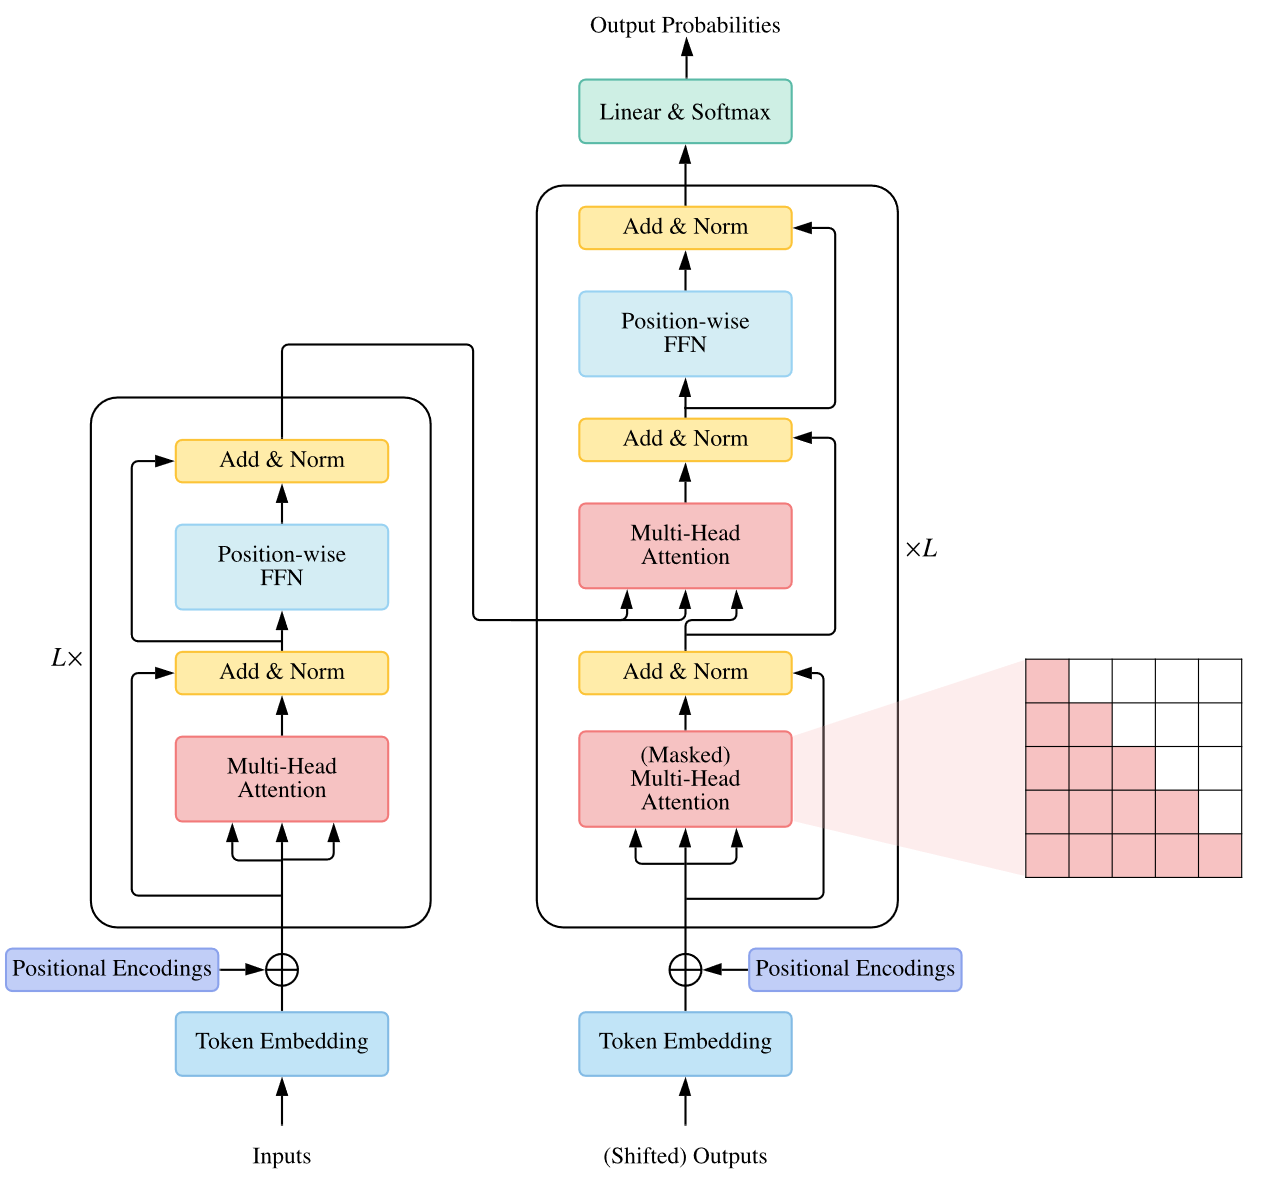
\includegraphics[width=0.8\linewidth]{images/transformer.png}
\caption[Transformers]{Transformer Architecture \cite[Figure 1, p. 3]{lin2022SurveyTransformers}} \label{fig:transformer}
\end{figure}


\subsection{Diffusion Probabilistic Models}
\label{ch:preliminaries-diffusionProbabilisticModels}

The \Glspl{ddpm} (from now on referred to as "diffusion model"), firstly introduced by \textcite{sohl-dickstein2015DeepUnsupervisedLearning}, is a generative modeling approach inspired by non-equilibrium statistical physics \cite{sohl-dickstein2015DeepUnsupervisedLearning}.
\textcite{ho2020DenoisingDiffusionProbabilistic} in their work, how diffusion models can successfully generate high-quality synthetic images.
This section will provide an explanatory introduction to the diffusion model concept, drawing heavily on the foundational work of \cite{ho2020DenoisingDiffusionProbabilistic}.
Although several other researchers have made notable advancements to diffusion probabilistic models, the work presented in \cite{sohl-dickstein2015DeepUnsupervisedLearning, ho2020DenoisingDiffusionProbabilistic} 
serves as the cornerstone upon which all subsequent improvements have been built.
Improvements and alternations made to \cite{ho2020DenoisingDiffusionProbabilistic} will be discussed in detail in \autoref{ch:relatedWork-diffusionModels}.

On a high level, the whole diffusion concept can be summarized as follows:

\begin{quotation}
  "The essential idea, (...) is to systematically and slowly destroy structure in a data distribution through an iterative forward diffusion process. 
  We then learn a reverse diffusion process that restores structure in data, yielding a highly flexible and tractable generative model of the data." \cite[p. 1]{sohl-dickstein2015DeepUnsupervisedLearning}
\end{quotation}

Formally, \cite{ho2020DenoisingDiffusionProbabilistic} defines diffusion models as a class of \glspl{lvm} of the form $p_\theta(x_0):= \int_{}^{}p_\theta(x_{0:T})dx_{1:T}$,
with $x_1, ..., x_T$ as latents of the same dimensionality as samples from the data distribution $x_0 \sim q(x_0)$.
Diffusion models consist of a forward process and a reverse process.
During the forward process, an initial data point $x_0$ is obtained from the data distribution $q(x_0)$.
In the forward process (also called diffusion process), a fixed \gls{mc} gradually adds noise to the data.
$T$ defines the number of noising steps and $x_1,...,x_T$ denotes the latent variables, \ie the noised versions of the original data, with $x_T$ being the fully noised version of the data \cite{ho2020DenoisingDiffusionProbabilistic}.
The amount of added (Gaussian) noise in each timestep varies depending on the current timestep, which is controlled by a variance schedule $\beta_1, ..., \beta_T \in (0,1)$ \cite{ho2020DenoisingDiffusionProbabilistic}.
The forward process is defined as:

\begin{equation}
  \label{eqn:forwards_1}
  \begin{align*}
    q(x_{1:T} | x_0) := \prod_{t=1}^T q(x_t | x_{t-1}), \quad
    q(x_t | x_{t-1}) := \mathcal{N}(x_t; \sqrt{1 - \beta_t} x_{t-1}, \beta_t I)
  \end{align*}
\end{equation}

For the variance schedule it holds that if $\beta_1 < \beta_2 < ... < \beta_T$ for $t\rightarrow\infty$, the final latent $x_t$ is isotropic Gaussian noise, \ie, $x_t \sim \mathcal{N}(0, \textbf{I})$, with identity matrix $\textbf{I}$ \cite{zbinden2022ImplementingExperimentingDiffusion}.
$\beta$ increases linearly in the original \gls{ddpm} approach \cite{ho2020DenoisingDiffusionProbabilistic} but was later improved to follow a cosine schedule \cite{nichol2021ImprovedDenoisingDiffusion}, improving the overall quality of the model.

\autoref{eqn:forwards_1} \cite{ho2020DenoisingDiffusionProbabilistic} shows how iteratively one noising step can be applied to get from $x_{t-1}$ to $x_t$ with $q(x_t | x_{t-1})$.
Through the use of a reparameterization (see \autoref{eqn:reparameterization}) and defining $\alpha := 1-\beta_t$ and $\overline{\alpha_t}:=\prod_{s=1}^{t}a_s$, 
the forward diffusion process from an unnoised input $x_0$ to a noised version at $t$ can be expressed as follows:

\begin{equation}
  \label{eqn:forwards_2}
  \begin{align*}
    q(x_t | x_0) \quad & := \mathcal{N}(x_t; \sqrt{\bar{\alpha}_t} x_0, (1 - \bar{\alpha}_t) \textbf{I})\\
    %  x_t &= \sqrt{\bar{\alpha}_t} x_0 + \sqrt{1 - \bar{\alpha}_t} \epsilon \textrm{, with } \epsilon\sim\mathcal{N}(0, \textbf{I})
  \end{align*}
\end{equation}

\autoref{eqn:forwards_2} \cite{ho2020DenoisingDiffusionProbabilistic} allows computing the forward noising from $x_0$ to any timestep $t$ within one computation step instead of iteratively applying noise over and over again.

During the reverse process, the goal is to learn the reverse distribution from noised data $x_t$ to slightly less noised data $x_{t-1}$, $q(x_{t-1}|x_t)$.
With bayes-theorem we can see that $q(x_{t-1}|x_t) = \frac{p(x_{t-1},x_t)}{p(x_t)}$, which means $q(x_{t-1}|x_t)$ depends on the marginal distribution of $x_t$, denoted as $p(x_t)$.
To calculate the marginal probability distribution $p(x_t)$ integration over all possible realizations of $x_{t-1}$ would be necessary, which would be computationally intractable \cite{capel2022MasterThesisDenoising}.
As a result, $q(x_{t-1}|x_t)$ is approximated by a neural network with learnable parameters $\theta$ that learns the joint distribution $p_{\theta}(x_{0:T})$.
$p_{\theta}(x_{0:T})$ is a \gls{mc}, defined in \autoref{eqn:reverse_1}, with the transitions defined in \autoref{eqn:reverse_2} \cite{capel2022MasterThesisDenoising, ho2020DenoisingDiffusionProbabilistic}.

\begin{equation}
  \label{eqn:reverse_1}
  \begin{align*}
    p_{\theta}(x_{0:T}) := p(x_T) \prod_{t=1}^T p_{\theta}(x_{t-1} | x_t),
  \end{align*}
\end{equation}

\begin{equation}
  \label{eqn:reverse_2}
  \begin{align*}
    p_{\theta}(x_{t-1}|x_t) := \mathcal{N}(x_{t-1}; \mu_{\theta}(x_t, t), \Sigma_{\theta}(x_t, t))
  \end{align*}
\end{equation}
    
While the mean $\mu_{\theta}(x_t, t)$ is learned by the neural network, the variance $\Sigma_{\theta}(x_t, t)$ stayed fixed in the initial work by \cite{ho2020DenoisingDiffusionProbabilistic} 
but was later in \textcite{nichol2021ImprovedDenoisingDiffusion} work a learnable parameter as well \cite{zbinden2022ImplementingExperimentingDiffusion}.

Like in \glspl{vae} (\autoref{ch:preliminaries-variationalAutoencoders}), the model is trained by minimizing its negative log-likelihood (= maximizing the log-likelihood) $-log(p_\theta(x_0))$.
$p_\theta(x_0)$ depends on all timesteps before $x_0$ and is, therefore, not tractable in practice \cite{zbinden2022ImplementingExperimentingDiffusion}.
As a solution, the variational lower bound on the negative log-likelihood can be computed \autoref{eqn:vlb}: %(ELBO)

\begin{equation}
  \label{eqn:vlb}
  \begin{align*}
    -log(p_\theta(x_0)) \leq -log(p_\theta(x_0)) + KL(q(x_{1:T}|x_0) \parallel p_\theta(x_{1:T}|x_0))
  \end{align*}
\end{equation}

The \gls{kl}-divergence (\autoref{eqn:kl-divergence}) is a non-negative measure of dissimilarity between two probability distributions. 
The right-hand side is reduced by minimizing the \gls{kl}-divergence as the objective function in the given inequality, leading to a smaller or equal left-hand side. 
Consequently, minimizing the \gls{kl}-divergence can only decrease the negative log-likelihood term on the left-hand side of the inequality. 
This implies that the objective function provides a lower bound on the log-likelihood and any improvement in minimizing the \gls{kl}-divergence will ultimately lead to an enhancement in this lower bound.
Rewriting $KL(q(x_{1:T}|x_0) \parallel p_\theta(x_{1:T}|x_0))$ to $log(\frac{q(x_{1:T})|x_0}{p_\theta(x_{1:T}|x_0)})$ and some reformulations (see \autoref{eqn:vlb2_appendix}) using bayes-rule results in \autoref{eqn:vlb2} leads to the following inequation \cite{ho2020DenoisingDiffusionProbabilistic}:

\begin{equation}
  \label{eqn:vlb2}
  \begin{align*}
    -log(p_\theta(x_0)) \leq log(\frac{q(x_{1:T})|x_0)}{p_\theta(x_{0:T})})
  \end{align*}
\end{equation}

\autoref{eqn:vlb2} is the variational lower bound that is minimized during training to optimize $-log(p_\theta(x_0))$.
With additional reformulations (see \autoref{eqn:vlb3_appendix}), the loss function can be derived as \cite{ho2020DenoisingDiffusionProbabilistic}:

\begin{equation}
  \label{eqn:vlb3}
  \begin{align*}
   \mathbb{E}\biggl[\underbrace{D_{KL}(q(x_{T}|x_0) \parallel p(x_T))}_{L_T} + \sum_{t>1}^{} \underbrace{  D_{KL}(q(x_{t-1}|x_t,x_0) \parallel p_\theta(x_{t-1}|x_t)) }_{L_{t-1}}  \underbrace{ -log p_\theta(x_0|x_1) }_{L_{0}}\biggr]
  \end{align*}
\end{equation}

$L_T$ consists of $q(x_{T}|x_0)$ and is a noising forward process that has no learnable parameters and $p(x_T)$ is Gaussian distributed noise.
If the forward process correctly destroys the data, $q(x_{T}|x_0)$ will converge to a standard Gaussian distribution as well and one can be confident that $L_T$ will be close to $0$.
Thus, $L_T$ will be neglected.

To $L_{0}$ can also be referred to as a "reconstruction term" \cite[p. 10]{luo2022UnderstandingDiffusionModels}.
\textcite{ho2020DenoisingDiffusionProbabilistic} initially use an independent discrete decoder to determine $L_{0}$, derived from $\mathcal{N}(x_0;\mu_0(x_1,1)\sigma^2_1,\textbf{I})$.
However, ultimately the authors decide to remove the term in favor of a simpler loss term, which leads to a simpler implementation and better quality \cite{ho2020DenoisingDiffusionProbabilistic}.

Inside $L_{t-1}$, one compares the target denoising step $q(x_{t-1}|x_t,x_0)$ that is also conditioned on the input $x_0$ with the approximated denoising step $p_\theta(x_{t-1}|x_t)$. %%%
Both terms have a closed-form solution (meaning they can be computed within a finite amount of standard computations) thanks to the conditioning on $x_0$ \cite{ho2020DenoisingDiffusionProbabilistic}:

\begin{equation}
  \label{eqn:lt-1_1}
  p_\theta(x_{t-1}|x_t)= \mathcal{N}(x_{t-1};\mu_\theta(x_t,t), \beta\textbf{I})
\end{equation}

\begin{equation}
  \label{eqn:lt-1_2}
q(x_{t-1}|x_t,x_0) = \mathcal{N}(x_{t-1};\tilde{\mu_t}(x_t,x_0), \tilde{\beta_t}\textbf{I})
\end{equation}

\autoref{eqn:lt-1_2} can be further simplified, considering that:
\begin{equation}
  \begin{align}
    &\tilde{\mu_t}(x_t, x_0) := \frac{\sqrt{\bar{\alpha}_{t-1}}\beta_t}{1 - \alpha_{\bar{t}}}x_0 +   \frac{\sqrt{\alpha_t}(1-\bar{\alpha}_{t-1})}{1 - \bar{\alpha}_{t}}x_t \quad \textrm{and }
    \tilde{\beta_t}:=\frac{1-\bar{\alpha}_{t-1}}{1-\bar{\alpha}_t}\beta_t \nonumber\\
  \end{align}
\end{equation}
    
\begin{equation}
  \begin{align}
    &x_t = \sqrt{\bar{\alpha}_{t}}x_0+\sqrt[]{1-\bar{\alpha}_t}\epsilon \quad\textrm{and }
    x_0 = \frac{1}{\sqrt{\bar{\alpha}_t}}(x_t-\sqrt[]{1-\bar{\alpha}_t}\epsilon) \nonumber\\
  \end{align}
\end{equation}

with $\beta$ being fixed by \cite{ho2020DenoisingDiffusionProbabilistic} and the mean $\tilde{\mu_t}$ is being further simplified to \autoref{eqn:lt-1_3} \cite{ho2020DenoisingDiffusionProbabilistic}:

\begin{equation}
  \begin{align}
    \label{eqn:lt-1_3}
    \tilde{\mu_t}(x_t, x_0) = \frac{1}{\sqrt{\bar{\alpha}_t}}(x_t - \frac{\beta_t}{\sqrt[]{1-\bar{\alpha}_t}}\epsilon)
  \end{align}
\end{equation}

which is just scaled random noise that is subtracted from $x_t$, the fully noised data.

Hence, the \gls{kl}-divergence in $L_{t-1}$ in \autoref{eqn:vlb2} ultimately measures the difference between the actual noise that was added ($\tilde{\mu_t}$ in \autoref{eqn:lt-1_3}) and the predicted noise from the neural network ($\mu_\theta$ in \autoref{eqn:lt-1_1}).
\textcite{ho2020DenoisingDiffusionProbabilistic} proposes the \gls{mse} between $\tilde{\mu_t}$ and $\mu_\theta$ as a loss function:

\begin{equation}
  \begin{align}
    \label{eqn:mse_loss}
    L_{t-1} = \mathbb{E}_q \left[ \frac{1}{2\sigma_t^2} \left\Vert \tilde{\mu}_t(x_t, x_0) - \mu_\theta(x_t, t) \right\Vert^2 \right] + C
  \end{align}
\end{equation}

The constant $C$ will be removed during training, as it does not depend on $\theta$ \cite{ho2020DenoisingDiffusionProbabilistic}.
By applying the same reparameterization that was done in \glspl{vae} (see \autoref{eqn:reparameterization}) to $\mu_\theta$, it can be reformulated in the following way:

\begin{equation}
  \begin{align}
    \label{eqn:mse_loss_2}
    \mu_\theta(x_t,t)= \frac{1}{\sqrt{\alpha_t}}(x_t - \frac{\beta_t}{\sqrt[]{1-\bar{\alpha}_t}}\epsilon_\theta(x_t,t)) 
  \end{align}
\end{equation}

With the reparameterization of \autoref{eqn:mse_loss_2}, the parametrization of what the model should predict in the reverse process (from $x_t$ to $x_{t-1}$) is moved. 
Instead of predicting the mean and variance of the reverse distribution ($p_\theta(x_{t-1}|x_t)$), \ie directly predicting the less noised data, 
the model predicts the noise $\epsilon$ that makes the difference between $x_{t-1}$ and ${x_t}$.
In other words, instead of predicting the new data directly, the model learns to predict what noise it needs to remove from the data \cite{capel2022MasterThesisDenoising}.
Ultimately, during sampling $x_{t-1}$ can be calculated by:

\begin{equation}
  \begin{align*}
    \label{eqn:xt-1}
    x_{t-1} = \frac{1}{\sqrt{\alpha_t}}\left(x_t - \frac{\beta_t}{\sqrt{1-\bar{\alpha}t}}\epsilon_{\theta}(x_t,t)\right) + \sigma_t z \textrm{,}\quad
    \textrm{with } \beta_t := 1-\alpha_t
  \end{align*}
\end{equation}

Where $z\sim\mathcal{N}(0,\textbf{I})$ is a random component that is added during the reverse process (except for $t=1$) to ensure the generation of diverse samples.

Substituting $\tilde{\mu_t}$ as in \autoref{eqn:lt-1_3} and $\mu_\theta$ as in \autoref{eqn:mse_loss_2} with some further simplification leads to:

\begin{equation}
  \begin{align*}
    \label{eqn:eqn:lt-1_4}
    L_{t-1} &= \mathbb{E}_{x_0,\epsilon} \left[  \frac{\beta^2_t}{2\sigma_t^2 \alpha_t (1-\bar{\alpha}_t)} ||\epsilon - \epsilon_\theta(x_t,t)||^2 \right] \\
    &= \mathbb{E}_{x_0,\epsilon} \left[  \frac{\beta^2_t}{2\sigma_t^2 \alpha_t (1-\bar{\alpha}_t)} ||\epsilon - \epsilon_\theta( \underbrace{\sqrt{\bar{\alpha}_t} x_0 + \sqrt{1-\bar{\alpha}_t}\epsilon}_{x_t}, t)||^2 \right]
  \end{align*}
\end{equation}


Ultimately, \textcite[p. 5]{ho2020DenoisingDiffusionProbabilistic} discovered that simplifying the loss term even further improves not only the sample quality but is also easier to implement.
\autoref{eqn:l_simple} shows the final simplified loss function $L_{simple}$:

\begin{equation}
  \begin{align*}
    \label{eqn:l_simple}
    L_{simple}(\theta) = \mathbb{E}_{t, x_0,\epsilon} \left[ ||\epsilon - \epsilon_\theta( \sqrt{\bar{\alpha}_t} x_0 + \sqrt{1-\bar{\alpha}_t}\epsilon, t)||^2 \right]
  \end{align*}
\end{equation}

\textcite{ho2020DenoisingDiffusionProbabilistic} state that this simplified loss version is a weighted variational bound, which down-weights the loss for small $t$'s, which corresponds to data point with only little added noise.
They further argue that this is actually beneficial for the model since learning small noise is not difficult. 
Therefore the model can focus more on the large $t$'s, where the denoising is more difficult \cite{ho2020DenoisingDiffusionProbabilistic}.

\autoref{alg:training} shows the full training algorithm, which will be realized by firstly randomly sampling a datapoint $x_0 \sim q(x_0)$ from the dataset, a timestep $t\sim Uniform(\{1, ..., T\})$ and some random Gaussian noise $\epsilon \sim \mathcal{N}(0, \textbf{I})$.
Afterward, the gradient step will then be performed according to \autoref{eqn:l_simple} using gradient descent.

\begin{algorithm}[T]
  \caption[Training algorithm]{Training \cite[p. 4]{ho2020DenoisingDiffusionProbabilistic}}
  \label{alg:training}
  \begin{algorithmic}
    \Repeat
    \State $x_0 \sim q(x_0)$
    \State $t\sim Uniform(\{1, ..., T\})$
    \State $\epsilon \sim \mathcal{N}(0, \textbf{I})$
    \State Take gradient descent step on
    \State \hskip1.5em $\nabla_\theta||\epsilon - \epsilon_\theta( \sqrt{\bar{\alpha}_t} x_0 + \sqrt{1-\bar{\alpha}_t}\epsilon, t)||^2$
    \Until converged
  \end{algorithmic}
\end{algorithm}


Sampling, on the other hand, follows \autoref{alg:sampling}, starting with sampling Gaussian noise $x_T$.
The Gaussian noise is then denoised in an iterative manner for $T$ timesteps according to \autoref{eqn:xt-1} until a new, noise-free datapoint $x_0$ is generated.

\begin{algorithm}[H]
\caption[Sampling algorithm]{Sampling algorithm \cite[p. 4]{ho2020DenoisingDiffusionProbabilistic}}
  \label{alg:sampling}
  \begin{algorithmic}
  \State $x_T \sim \mathcal{N}(0, \mathbf{I})$
  \For{$t = T, \dots, 1$}
  \State $z \sim \mathcal{N}(0, \mathbf{I})$ if $t > 0$ else $z = 0$
  \State $x_{t-1} = \frac{1}{\sqrt{\alpha_t}}\left(x_t - \frac{\beta_t}{\sqrt{1-\bar{\alpha}t}}\epsilon_{\theta}(x_t,t)\right) + \sigma_t z$
  \EndFor
  \State \Return $x_0$
  \end{algorithmic}
\end{algorithm}

In summary, \cite{ho2020DenoisingDiffusionProbabilistic} introduced \gls{ddpm} based on the work of \cite{sohl-dickstein2015DeepUnsupervisedLearning}.
Their diffusion model is based on a \gls{mc} and consists of the forward noising and the backward denoising part.
During the forward process, a timestep $t$ is sampled and the raw input data $x_0$ is noised accordingly using \autoref{eqn:forwards_2}.
A function approximator (usually a neural network) with learnable parameters $\theta$ tries to remove the noise by predicting the noise that was added during the forward process.
This difference between the actual noise $\epsilon$ and the predicted noise $\epsilon_{\theta}$ is used as a loss function (\autoref{eqn:l_simple}) to perform gradient descent.
Once the training is finished, and the model converges, new synthetic data can be generated during sampling.
In the sampling process, Gaussian noise can be sampled, and the model progressively denoises the sample for $T$ timesteps until a new, denoised datapoint $x_0$, is generated.


\subsection{Multinomial Diffusion}
\label{ch:multinomial}
The \gls{ddpm} apprach uses a Gaussian diffusion process, designed to operate in continuous space \cite{kotelnikov2022TabDDPMModellingTabular}.
However, many different data types are of categorical nature, where the Gaussian noising process proposed in \autoref{ch:preliminaries-diffusionProbabilisticModels} is not applicable.
As a response, \textcite{hoogeboom2021ArgmaxFlowsMultinomial} introduced multinomial diffusion, "a diffusion model directly defined on categorical variables" \cite[p, 3]{hoogeboom2021ArgmaxFlowsMultinomial}.

\cite{hoogeboom2021ArgmaxFlowsMultinomial} defines the multinomial diffusion process in the following way:

\begin{equation}
  \begin{align*}
    \label{eqn:mul_diff1}
    q(x_{t}|x_{t-1}) = \mathcal{C}(x_t|(1-\beta_t)x_{t-1}+\beta_t/K)
  \end{align*}
\end{equation}


The term $\beta_t$ denotes the likelihood of swapping the current categorical value with a different one. 
Essentially, it is deciding how much random variation, or "noise", is introduced.
This noise is based on a categorical uniform distribution, which means that it considers all available categories equally when picking a random value \cite{hoogeboom2021ArgmaxFlowsMultinomial}.
Furthermore, $\mathcal{C}$ denotes a categorical distribution and $x_t$ is represented in a \gls{oh} encoded categorical vector format with $K$ different classes, $x_t\in\{0,1\}^K$ \cite{hoogeboom2021ArgmaxFlowsMultinomial}.

The noising step from $x_0$ to any noised version $x_t$ can be expressed as:

\begin{equation}
  \begin{align*}
    \label{eqn:mul_diff2}
    q(x_{t}|x_{0}) = \mathcal{C}(x_t|\overline{\alpha}_tx_{0}+(1-\overline{\alpha}_t)/K)
  \end{align*}
\end{equation}

with $\alpha_t = 1-\beta_t$ and $\overline{\alpha}_t = \prod_{\tau=1}^{t}\alpha_\tau$.
Uniform noise is added over the $K$ classes in each timestep.
If $(1-\beta_t)$ is large, the model is likely to retain the previous category from $x_{t-1}$. 
Likewise, if $(1-\beta_t)$ is small, the model will rely more on sampling a random category from a uniform distribution over all categorical values for the variable.

\cite{hoogeboom2021ArgmaxFlowsMultinomial} derives from \autoref{eqn:mul_diff1} and \autoref{eqn:mul_diff2} the categorical posterior:

\begin{equation}
  \begin{gathered}
  \label{eqn:mul_diff3}
  q(x_{t-1}|x_t, x_{0}) = \mathcal{C}(x_{t-1}|\theta_{post}(x_t,x_0)),\textrm{ where } \theta_{post}(x_t,x_0)=\tilde{\theta}/\sum_{k=1}^{K}\tilde{\theta}_k \\
  \textrm{and } \tilde{\theta} = \left[\alpha_tx_{t}+(1-\alpha_t)/K \right] \odot \left[\overline{\alpha}_{t-1}x_{0}+(1-\overline{\alpha}_{t-1})/K \right]
  \end{gathered}
\end{equation}

\cite{hoogeboom2021ArgmaxFlowsMultinomial} argues, that predicting the added noise, as in \cite{ho2020DenoisingDiffusionProbabilistic},
is difficult, and instead the authors predict a probability vector for $\hat{x_0}$ from $x_t$.
The reverse distribution $p_\theta(x_{t-1}|x_t)$ is realized in the form of $q(x_{t-1}|x_t,\hat{x_0})$ where $\hat{x_0}=\mu(x_t, t)$ is predicted by the model and tries to approximate $x_0$ \cite{hoogeboom2021ArgmaxFlowsMultinomial}.
Hence:

\begin{equation}
  \begin{align*}
    \label{eqn:mul_diff4}
    p(x_0|x_1) = \mathcal{C}(x_0|\hat{x}_0) \textrm{ and } p(x_{t-1}|x_t) =  \mathcal{C}(x_{t-1}|\theta_{post}(x_t, \hat{x}_0)) \textrm{ where } \hat{x}_0=\mu(x_t,t)
  \end{align*}
\end{equation}

In other words, determining the categorical value assigned to $x_{t-1}$ (or $x_0$ in the last step) is based on the predicted probabilities $\hat{x}_0$ produced by the model.


The loss function in terms of \gls{kl}-divergence (\autoref{eqn:vlb3}) can be computed with \autoref{eqn:mul_diff3} and \autoref{eqn:mul_diff4}:

\begin{equation}
  \begin{align*}
    \label{eqn:mul_diff5}
    L_{t-1}&=\text{KL}\Big(q(x_{t-1}|x_t, x_0)\big\vert\big\vert p(x_{t-1}|x_t)\Big) = \text{KL}\Big(\mathcal{C}(\theta_{post}(x_t, x_0))\big\vert\big\vert \mathcal{C}(\theta_{post}(x_t, \hat{x}_0))\Big) \textrm{ and}\\
    L_{0} &= -logp(x_0|x_1) = \sum_{k}^{}x_{0,k}log\hat{x}_{0,k}
  \end{align*}
\end{equation}

Like in \cite{ho2020DenoisingDiffusionProbabilistic}, $L_{t}$ has no learnable parameters and will be omitted.


%-------------------------------------------------------------------------
\section{Evaluation of Synthetic Tabular Data}
\label{ch:preliminaries-evaluationOfSyntheticTabularData}

A proper evaluation of the generated synthetic dataset is required to measure the effectiveness of the synthetic tabular data generation model.
This evaluation is no trivial task due to the complexity and challenges of tabular data discussed in \autoref{ch:preliminaries-dataSynthesis-tabularData}.
Other data modalities, like images, are usually much easier to evaluate, for example, through human inspection \cite{chundawat2022UniversalMetricRobust}. 
This is not the case for tabular data, where various factors need to be considered during evaluation.
\textcite[p. 6]{goncalves2020GenerationEvaluationSynthetic} identified two major dimensions that need to be considered during the evaluation, "data utility" and "information disclosure".
The former dimensionality focuses on the quality of the synthetic data regarding the usefulness and statistical similarity.
A synthetic dataset should have the same statistical and practical properties as its real counterpart from which it was generated, so it is helpful in practice and could be used as a substitute.
The latter focuses on the amount of information carried over from the original dataset since the synthetic dataset should not just be a copy of the real dataset.
Hence, it is realized by privacy measures that capture how much information of the real dataset is disclosed in the synthetic dataset \cite{goncalves2020GenerationEvaluationSynthetic}.
\textcite[p. 2]{little2021GenerativeAdversarialNetworksa} highlights that these two evaluation aspects, "high data utility" and "low disclosure risk", are two "competing interests" that need to be balanced.
This section will present different ways to evaluate synthetic tabular data, each focusing on a different evaluation aspect.
\cite{elemam2020SevenWaysEvaluate} identifies seven ways to evaluate synthetic data's utility aspect.
However, in the literature and in practice, only a few approaches are used and will be presented in greater detail.
Firstly, statistical similarity (data utility) will be presented, followed by machine learning efficacy (data utility) and privacy evaluation methods (information disclosure).
Lastly, additional evaluation methods are shortly listed, and a proposed "similarity score" as a unified metric is presented.

\subsection{Statistical Evaluation}
\label{ch:preliminaries-statisticalEvaluation}

Various different metrics can be used to measure the statistical similarity between a synthetic dataset and the corresponding real dataset.
As a start, synthetic data should have similar basic statistical measures.
For example, \cite{delcarmenrodriguez-hernandez2017DataGenCARSGeneratorSynthetic} compares different statistical properties of the original and synthetic data. 
The authors include computing the mean, standard deviation, proportion of unique values, and the number of distinct values for each attribute.

\cite{goncalves2020GenerationEvaluationSynthetic} proposes multiple more complex statistical measures that go beyond the comparison of single values, like the mean or standard deviation.
The \gls{kl}-divergence or its extension the Jensen-Shannon distance \cite{zhao2022CTABGANEnhancingTabular} can be calculated between a pair of probability distributions from the real and synthetic dataset \cite{goncalves2020GenerationEvaluationSynthetic, li2022TTSGANTransformerbasedTimeSeries}.
While this measures the similarity for one variable, or column, of the data only, correlations between multiple pairs of variables can also be measured using the \gls{pcd} \cite{goncalves2020GenerationEvaluationSynthetic}.
This metric evaluates the extent to which the synthetic dataset maintains the same inter-column relationships as those present in the original dataset.
Another measurement is the support-coverage score \cite{goncalves2020GenerationEvaluationSynthetic}.
The support-coverage metric deals with the mathematical support of the variables. 
More specifically, it assesses the similarity or identity between the range of potential values in the synthetic dataset and those in the original dataset.

\subsection{Machine Learning Efficacy}
\label{ch:preliminaries-machineLearningEfficacy}

The machine learning efficacy (also referred to as "machine learning utility" \cite{zhang2021GANBLRTabularData} or "cross classification" \cite{goncalves2020GenerationEvaluationSynthetic}) is an approach that measures the utility of synthetic data. 
It has been used in a variety of works \cite{zhao2022CTABGANEnhancingTabular, xu2019ModelingTabularData, zhang2021GANBLRTabularData, bourou2021ReviewTabularData, ge2021KaminoConstraintawareDifferentially}.
This metric investigates whether "it is possible to replace the real with generated data to solve problems using Machine Leaning models" \cite[p. 7]{bourou2021ReviewTabularData}.
A set of classification models (for example decision trees, regression models, neural networks and more) are evaluated in a classification or regression task.
\cite[p. 7]{goncalves2020GenerationEvaluationSynthetic} highlights two distinct ways to perform the machine learning efficacy:
\begin{enumerate}
  \item "CrCl-RS": train a model on real data and test it on hold-out data (test set) from both real and synthetic datasets.
  \item "CrCl-SR": train a model on synthetic data and test it on hold-out data from both real and synthetic datasets.
\end{enumerate}
\cite{goncalves2020GenerationEvaluationSynthetic} argues that the former is useful to evaluate if statistical properties are similar between real and synthetic datasets
and that the latter allows confirming whether "scientific conclusions drawn from (...) models trained on synthetic datasets can safely be applied to real datasets" \cite[p. 7]{goncalves2020GenerationEvaluationSynthetic}.
The performance of the classification models itself is based on commonly used metrics for classification/regression tasks, such as the f1-score or \gls{rmse}-score \cite{bourou2021ReviewTabularData, chundawat2022UniversalMetricRobust}.
It is important to mention that there is no universally accepted way to perform this machine learning efficacy, yet, as it is implemented differently throughout the literature.
For example, \cite{zhao2022CTABGANEnhancingTabular} makes use of five models and calculates five different metrics, 
\cite{ge2021KaminoConstraintawareDifferentially} on the other hand, uses nine different models but calculates only three different metric scores.
Moreover, \cite{kunar2021DTGANDifferentialPrivatea} uses four models with four metrics, and \cite{kim2021OCTGANNeuralODEbased} uses three models on only one metric.
In addition to the various models and metric scores used, each model can have different hyperparameters.
For example, \cite{kunar2021DTGANDifferentialPrivatea} uses the default hyperparameters\footnote{from the scikit library \cite{scikit-learn}} for all models and 
\cite{kim2021OCTGANNeuralODEbased} chooses the hyperparameters that show the best performance in a cross-validation hyperparameter tuning.
Lastly, the different synthetic data generation models might use different datasets to compute their machine learning efficacy scores.
Even though most of the generation approaches have adopted the \textit{CrCl-SR} \cite{goncalves2020GenerationEvaluationSynthetic} method to calculate the machine learning efficacy score,
the aforementioned variabilities in terms of metrics- and model-choice make it hard to compare the performance across the different generative models using the machine learning efficacy.
%[TODO: ACC, F1 und ROC-AUC erklären? oder eher im concept part?]

\subsection{Privacy Evaluation}
\label{ch:preliminaries-evaluationOfSyntheticTabularData-privacyEvaluation}
\textcite[p. 7f.]{goncalves2020GenerationEvaluationSynthetic} discussed two types of privacy aspects that should be evaluated, "membership disclosure" and "attribute disclosure".
While the former is concerned with whether an individual from the original dataset can be identified in the synthetic dataset, the latter is concerned with the possibility of inferring actual values for an attribute of the original dataset, given the synthetic dataset.
To measure the \textit{membership disclosure}, \cite{goncalves2020GenerationEvaluationSynthetic} proposes calculating the distance of synthetic datapoints to real datapoints.
If this distance is smaller than a specific value, the synthetic datapoint is considered to be present in the original dataset.
The distance measure used by \cite{goncalves2020GenerationEvaluationSynthetic} was the \textit{Hamming-distance}, but this could be replaced with a similarity measure of choice, depending on the data.
\textit{Attribute disclosure} could be measured by testing if a potential attacker could infer unknown attributes, given a subset of known attributes by using a k-nearest neighbors algorithm \cite{goncalves2020GenerationEvaluationSynthetic}.
These privacy measures are especially prominent and essential in the context of medical data, that usually has sensitive information \cite{goncalves2020GenerationEvaluationSynthetic, choi2017GeneratingMultilabelDiscrete}.

To ensure privacy is granted, research towards including \gls{dp} \cite{dwork2008DifferentialPrivacySurvey} in the model has been made, \eg in \cite{xie2018DifferentiallyPrivateGenerative, jordon2018PATEGANGeneratingSynthetic, torfi2022DifferentiallyPrivateSynthetic}.
\gls{dp} is a concept in the field of data privacy that aims to protect the privacy of individuals while still allowing useful information to be extracted from data \cite{dwork2008DifferentialPrivacySurvey}. 
It provides a mathematical framework for measuring the privacy risk associated with releasing data and designing algorithms that minimize this risk \cite{dwork2008DifferentialPrivacySurvey, zhao2022CTABGANEnhancingTabular}.
\gls{dp} can be achieved by injecting noise to the gradients during the learning process \cite{xie2018DifferentiallyPrivateGenerative}.

\subsection{Additional Evaluation Methods}
\label{ch:preliminaries-evaluationOfSyntheticTabularData-otherMetrics}

There are several other ways to evaluate synthetic data that do not fall directly into the categories above but are worth mentioning.
\cite{elemam2020SevenWaysEvaluate} mentioned that the quality of synthetic data can be determined by a domain expert, 
who is familiar with how data in the given domain should look.
The expert could be asked to differentiate a set of synthetic data samples from a set of real data samples, and the accuracy could be measured.
However, this metric is not only highly dependent on the individual expert it is also very time-consuming and hardly viable in practice.

Another measure proposed by \cite{elemam2020SevenWaysEvaluate} is to compute aggregations and statistics of the synthetic data and compare it to publicly available known statistics and aggregations that are about the same topic.
If the synthetic is good, it would "tell the same story as the public data" \cite[p. 58]{elemam2020SevenWaysEvaluate}.

To determine the stability of the generative model, \cite{elemam2020SevenWaysEvaluate} proposes that the model could be used to generate not a single synthetic dataset but multiple.
Evaluation (\eg using a statistical measure such as in \autoref{ch:preliminaries-statisticalEvaluation}) is then performed on all synthetic datasets, and averages are calculated.
This repetition should highlight if the generative model has learned any form of bias or instability, which is not desirable \cite{elemam2020SevenWaysEvaluate}.

Lastly, \cite{hernandez2022SyntheticDataGeneration} proposes a set of resemblance techniques to measure the similarity of the synthetic data to the real data.
Most of \cite{hernandez2022SyntheticDataGeneration} proposed methods have already been mentioned and fall into one of the categories above, such as "consultation with [...] experts" or computing "correlation coefficients" \cite{hernandez2022SyntheticDataGeneration}.
Another viable way to quickly get an indication of how well the similarity is, is through visualization techniques.
\cite{hernandez2022SyntheticDataGeneration} proposes dimensionality reduction techniques like \gls{pca}, histograms of attributes, and correlation matrices can be computed and visualized.
With this visualization, a human can quickly determine, if the visualizations produced by the synthetic data resemble those of the real data.
For example, this type of visual evaluation was performed in the works \textcite{li2022TTSGANTransformerbasedTimeSeries, leminh2021AirGenGANbasedSynthetica, mckeever2020SynthesisingTabularDatasets}.


\subsection{Similarity Score}
\label{ch:preliminaries-similarityScore}
Given the previous sections, one can see that various evaluation techniques exist.
This variety is problematic for comparing the approaches to generate synthetic data, as there is no universally accepted metric or benchmark to compare the techniques \cite{hernandez2022SyntheticDataGeneration, chundawat2022UniversalMetricRobust}.
\textcite{brenninkmeijer2019GenerationEvaluationTabular} proposes a similarity score to address this issue by providing a single score that aggregates different metrics used throughout the literature. 
It consists of the average of five different similarity metrics that cover different aspects of the data. These are:
\begin{itemize}
  \item $S_{basic}$: compares the mean and standard deviation of the real and synthetic dataset using $Spearman's$ $\rho$ \cite{lane2003IntroductionStatistics} correlation per column.
  \item $S_{corr}$: calculates correlations/associations between the columns within the real and synthetic dataset using a correlation/association matrix. 
  Different statistical correlation measures are used to measure the correlation between columns of different data types \cite[p. 37]{brenninkmeijer2019GenerationEvaluationTabular}.
  Pearson's correlation for two continuous columns, correlation ratio between continuous and categorical, and Theil's U for two categorical \cite{brenninkmeijer2019GenerationEvaluationTabular, lane2003IntroductionStatistics}.  
  Ultimately, the matrices are compared using Pearson correlation $\rho_{pearson}$.
  \item $S_{mirr}$: the mirror column association score is similar to $S_{corr}$, but instead of comparing the correlations occurring between columns within the dataset,
  the metric compares whether the same columns in the real, and synthetic dataset correlate.
  This is done for each column and the average score is calculated.
  \item $S_{pca}$: measures whether the dimensionality reduction of the real and synthetic dataset through \gls{pca} is similar.
  Five principal components are computed for each dataset, and the average error in percentage between both \glspl{pca} is calculated using the mean absolute percentage error.
  \item $S_{est}$: is a machine learning efficacy similarity score. Four different models are chosen, depending on whether the dataset is a classification or regression dataset, and performance metric averages are computed.
  The root mean squared error and F1 score for regression or classification tasks respectively is chosen as performance metric.
\end{itemize}


\textcite{chundawat2022UniversalMetricRobust} propose TabSynDex, a single similarity score based upon combining multiple scores covering different aspects of data similarity like in the works of \cite{brenninkmeijer2019GenerationEvaluationTabular}.
In their work, they point out weaknesses of the similarity score proposed by \textcite{brenninkmeijer2019GenerationEvaluationTabular}.
For example, they criticized the usage of correlations as a primary similarity metric for basic statistical measures.
The issue with this is, that even if real and synthetic data's statistics are close but don't follow the same pattern, they don't correlate and their similarity will be considered to be very low.
As a result, even when comparing two parts of the same dataset, the similarity can appear low, which is contradictory since they come from the same distribution.
As a consequence, they propose the following similarity metrices:

\begin{description}
  \item[Basic statistical measure:]
  Computes basic statistics of the data for each column, namely mean, median and standard deviation, and calculates the relative error between the real and fake columns:
  
  \begin{equation}
    \begin{align*}
      \label{eqn:rel_err}
      e=\frac{1}{N} \bigg| \frac{R_i-F_i}{R_i} \bigg| 
      \end{align*}
  \end{equation}

  with $R_i$ and $F_i$ denoting the statistical measure of column $i$ for the real and synthetic data, respectively.
  The score for each metric is calculated as follows:
  $$s_m = 1-\frac{e^m_1+e^m_2+...+e^m_n}{n} \textrm{, with }m \in \{mean, median, std\}$$
  where n is the number of columns.
  The final score will be calculated as
  \begin{equation}
    \begin{align*}
      \label{eqn:s_basic}
      S_{basic} = \frac{s_{mean}+s_{median}+s_{std\_dev}}{3}
      \end{align*}
  \end{equation}


  \item[Log-transformer Correlation:]
  Compares the correlations between columns within the datasets to compute two matrices with $n^2$ values for $n$ columns.
  Correlations are calculated depending on the data type, like in \cite{brenninkmeijer2019GenerationEvaluationTabular}.
  The matrix entries are also log-transformed to account for the issue of very small values in the correlation matrix of real data, which can result in higher relative error values when compared to the correlation matrix for generated data, even if both correlations are nearly zero. 
  The log transformation helps to rescale the values and provide a more accurate comparison between the correlation matrices of real and generated data.
  \autoref{eqn:s_corrl} defines the correlation score, where $sln(x) = sign(x)ln(|x|)$ and $r_{i,j}, s_{i,j}$ indicating the matrix entries of the real and synthetic data.
  $sign(x)$ is defined as
  $$\textrm{sign}(x) = \begin{cases}1 & \text{if } x > 0 & -1 & \text{if } x < 0 & 0 & \text{if } x = 0\end{cases}$$
  which results in the final score:
  
  \begin{equation}
    \begin{align}
      \label{eqn:s_corrl}
      S_{corrl} = 1-\frac{1}{n^2-n} \sum_{i=1}^{n}\sum_{j=1_{j \neq i}}^{n} \bigg| \frac{sln(r_{i,j})- sln(s_{i,j})}{sln(r_{i,j})}\bigg| 
      \end{align}
  \end{equation}

  \item[Propensity Mean Squared Error:]
  Is used to "robustly discriminate between real and synthetic data" \cite[p. 3]{chundawat2022UniversalMetricRobust}.
  It is based upon the work of \textcite{snoke2018GeneralSpecificUtility}, who propose the use of the \gls{pmse} in the context of synthetic data generation.
  The \gls{pmse} is computed by combining a set of samples from the real and synthetic dataset and adding a label $Y$ to each entry, 
  indicating whether the given sample stems from the real or the synthetic dataset.
  A logistic regression model is trained to predict probabilities $\hat{p}_i$ for each sample $i$ for it being a synthetic data sample.
  The \gls{pmse} is calculated as:
  $$pMSE = 1-\frac{1}{N} \sum_{i=1}^{n}(\hat{p}_i-c)^2$$

  with $c=N_{syn}/(N_{real}+N_{syn})$ indicating the proportion of synthetic samples.
  
  For a similarity score, \textcite{chundawat2022UniversalMetricRobust} ultimately uses the \gls{pmse}-ratio as a final measure.
  For this, the so-called null distribution of \gls{pmse} is required \cite[p. 668]{snoke2018GeneralSpecificUtility}.
  This null distribution is essentially derived under the assumption of perfect synthesis, where the synthetic data are generated from the same model that produced the original data. 
  This creates a baseline for comparing the quality of synthetic data, serving as a reference point to evaluate the effectiveness of different synthetic data generation methods \cite{snoke2018GeneralSpecificUtility}.
  Essentially, it computes the expected value of \gls{pmse} when the real and synthetic data are indistinguishable.
  It is calculated as \cite{snoke2018GeneralSpecificUtility,chundawat2022UniversalMetricRobust}:
  $$\mathbb{E}(pMSE_0) = \frac{(k-1)(1-c)^2c}{N}$$
  with the logistic regression model having $k$ parameters (including bias) \cite{chundawat2022UniversalMetricRobust}.
  \cite{chundawat2022UniversalMetricRobust} improves the original metric as introduced in \cite{snoke2018GeneralSpecificUtility} further through the introduction
  of a value $\alpha$ that can be chosen task-specific and helps standardization of the score to $[0,1]$ (the authors' default is set to $\alpha=1.2$)
  The final score is calculated as 
  \begin{equation}
    \begin{align*}
      \label{eqn:s_pmse}
      S_{pMSE} = \alpha^{|1-\frac{pMSE}{\mathbb{E}(pMSE_0)}|}
      \end{align*}
  \end{equation}
  that calculates the ration of $pMSE$ and $pMSE_0$.
  Hence, the closer the ratio is to 1, the more indistinguishable the synthetic data is from the real data \cite{chundawat2022UniversalMetricRobust}.
  

  \item[Regularized Support Coverage:]
  Measures how well a synthetic dataset covers the variables in a real dataset. 
  For a single variable, the score is calculated as the average of the number of samples in each category in the fake data 
  divided by the number of samples in the corresponding category in the real data, multiplied by a scaling factor. 
  It penalizes the score more if rare categories are not well-represented. 
  
  Mathematically, the score for a single variable or column $c$ is calculated as follows:

  $$ s_{cr} = \frac{1}{n_{cat}} \sum_{i=1}^{n_{cat}} \frac{n^s_i}{n^r_i} \cdot scaling~factor $$

  Where $n_{cat}$ is the number of categories for a variable, $n^s_i$ is the number of samples in that category in the synthetic data, $n^r_i$ is the corresponding number of samples in the real data, and the scaling factor is $N_{real}/N_{syn}$ \cite{chundawat2022UniversalMetricRobust}.
  The authors limit the $S_{cr}$ score to a predefined $\beta$ value (the authors' default is set to $\beta=2$), to account for the potential for $s_{cr}$ to become very sensitive to $n^s_i$, if $n^r_i$ is very small \cite{chundawat2022UniversalMetricRobust}.

  The final $S_{cr}$ score is calculated as the average of the score for each column \cite{chundawat2022UniversalMetricRobust}:

  \begin{equation}
    \begin{align*}
      \label{eqn:s_cr}
      S_{cr} = \frac{1}{n} \sum_{i=1}^{n} s_{cr_i}
      \end{align*}
  \end{equation}



  \item[Machine Learning Efficacy:]
  Is a metric to indicate how valuable the synthetic data is in a machine learning scenario (see \autoref{ch:preliminaries-machineLearningEfficacy}).
  \cite{chundawat2022UniversalMetricRobust} adopts the proposed metrics and models by \cite{brenninkmeijer2019GenerationEvaluationTabular} that differentiates the chosen set of models and metric based on
  if the dataset contains a classification or regression target.
  The models include \textit{Random Forest-}, \textit{Lasso-}, \textit{Ridge-} and \textit{ElasticNet-Regression} for regression tasks and \textit{Logistic Regression-}, \textit{Random Forest-},  \textit{Decision Tree-} and an \textit{\gls{mlp}-classifier} for classification tasks \cite{brenninkmeijer2019GenerationEvaluationTabular, chundawat2022UniversalMetricRobust}.
  For each model, two versions are trained, one trained on synthetic and one trained on real training data.
  Their performance is tested on both the real and synthetic targets using the F1-score or \gls{rmse}-score.
  For each model, the relative error (\autoref{eqn:rel_err}) is calculated between the metric results of the model that was trained on real data and the model that was trained on synthetic data.
  The final score is the average performance error for all four models:

  \begin{equation}
    \begin{align*}
      \label{eqn:s_ml}
      S_{ml} = 1-\frac{e_{m1}+e_{m2}+e_{m3}+e_{m4}}{4}
      \end{align*}
  \end{equation}
  where $e_{mi}$ is the error for the $i^{th}$ model \cite{chundawat2022UniversalMetricRobust}.
\end{description}

\item[Similarity Score:]
The final unified metric, named TabSynDex, is the average of all scores mentioned above and is described in \autoref{eqn:tabsyndex} \cite{chundawat2022UniversalMetricRobust}:

\begin{equation}
  \begin{align*}
    \label{eqn:tabsyndex}
    TabSynDex = \frac{S_{basic}+S_{corrl}+S_{pMSE}+S_{cr}+S_{ml}}{5}
    \end{align*}
\end{equation}
